\chapter{Prototipação das telas}
\label{prototipação}
% ----------------------------------------------------------
A seguinte seção apresentará as figuras referentes a prototipagem de alta fidelidade do projeto \gls{ifriends}. Para a prototipação levou-se em consideração, dois estados, sendo eles o do usuário com \textit{login} e o do usuário sem \textit{login}. 

%--------------------------------------------------------------
\section{Friend sem login}
%--------------------------------------------------------------
Quando um usuário externo ou até mesmo um \gls{friend} que ainda não tenha cadastro na aplicação decidir visualizar ou conhecer a comunidade, ele pode, mas terá algumas funcionalidades bloqueadas, podendo apenas visualizar o sistema.

Dessa forma, a \autoref{cadastro} representa a página de cadastro, na qual o \gls{friend} efetua seu cadastro.

\begin{figure}[htb]
\centering
\caption{\label{cadastro} Página de cadastro}
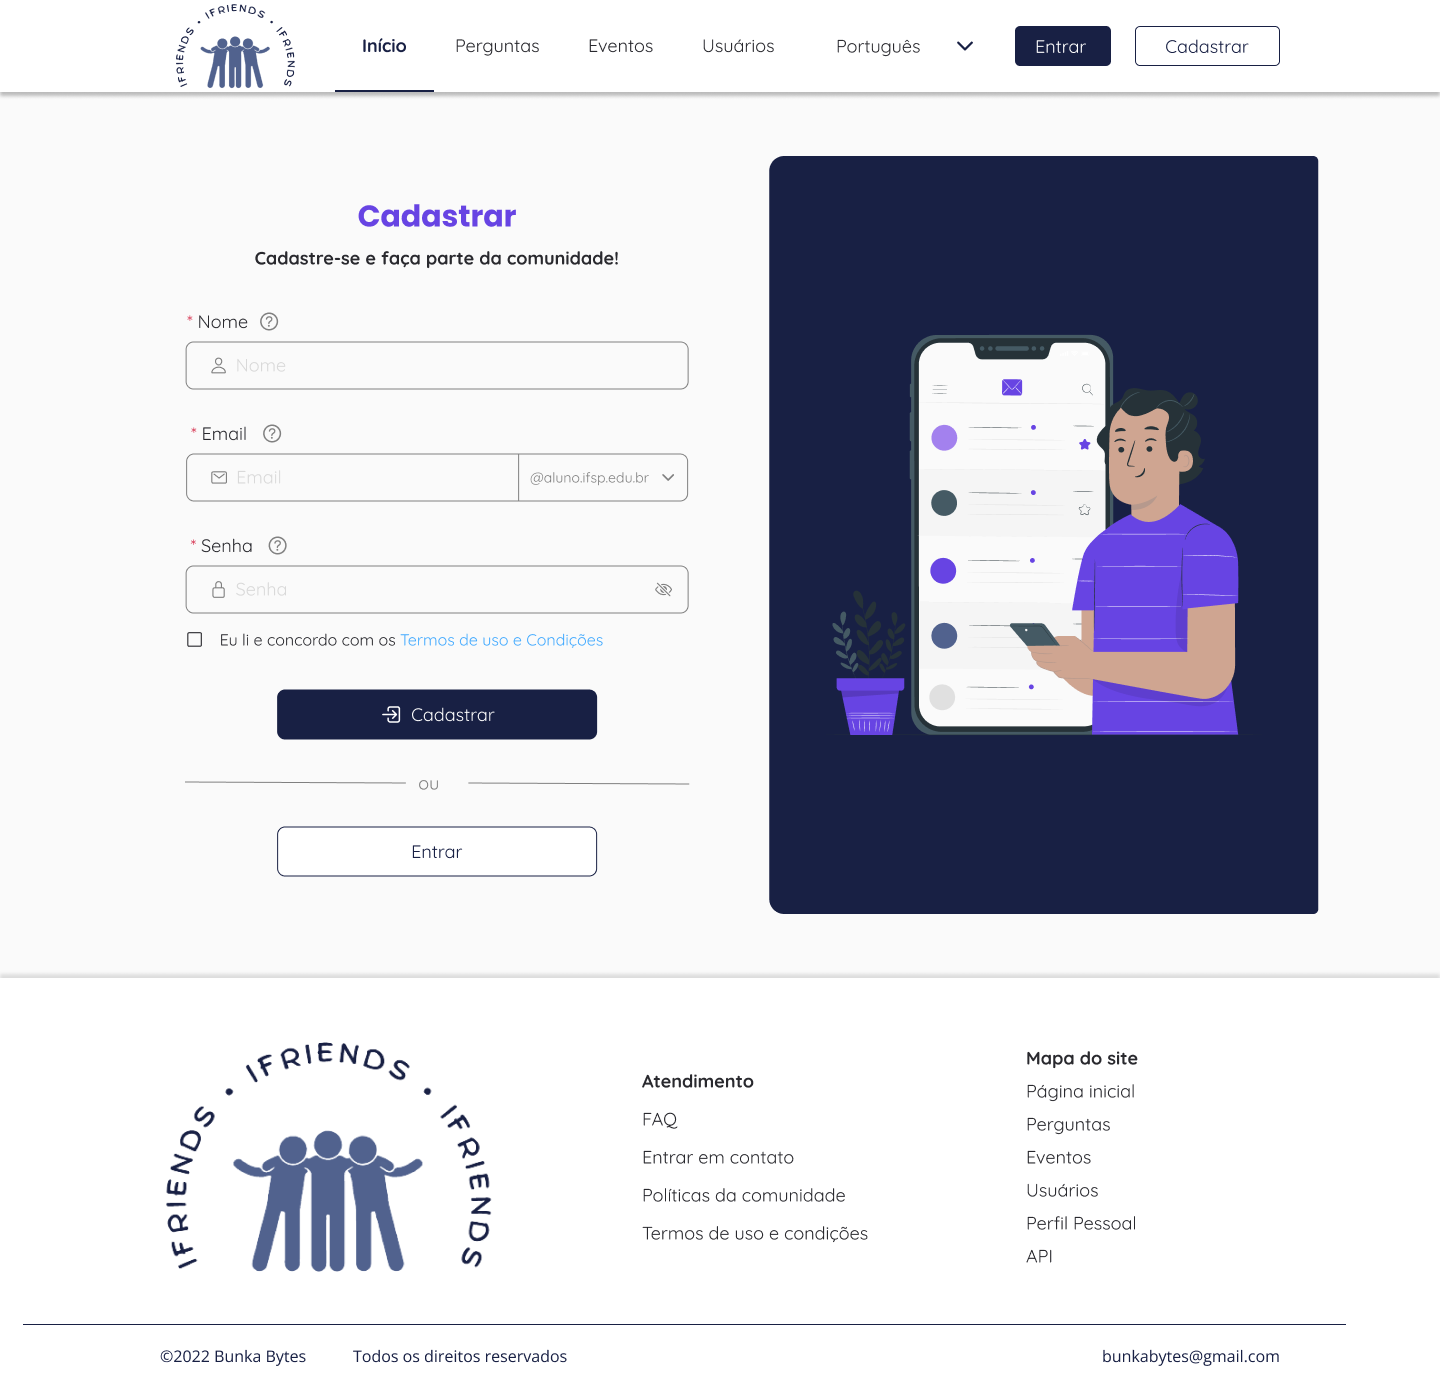
\includegraphics[width=0.8\textwidth]{anexos/Imagens_Prototipo/intro/cadastro.png}
\fonte{Os autores.}
\end{figure}
\FloatBarrier

A \autoref{login} representa a página de login. 

\begin{figure}[htb]
\centering
\caption{\label{login} Página de login}
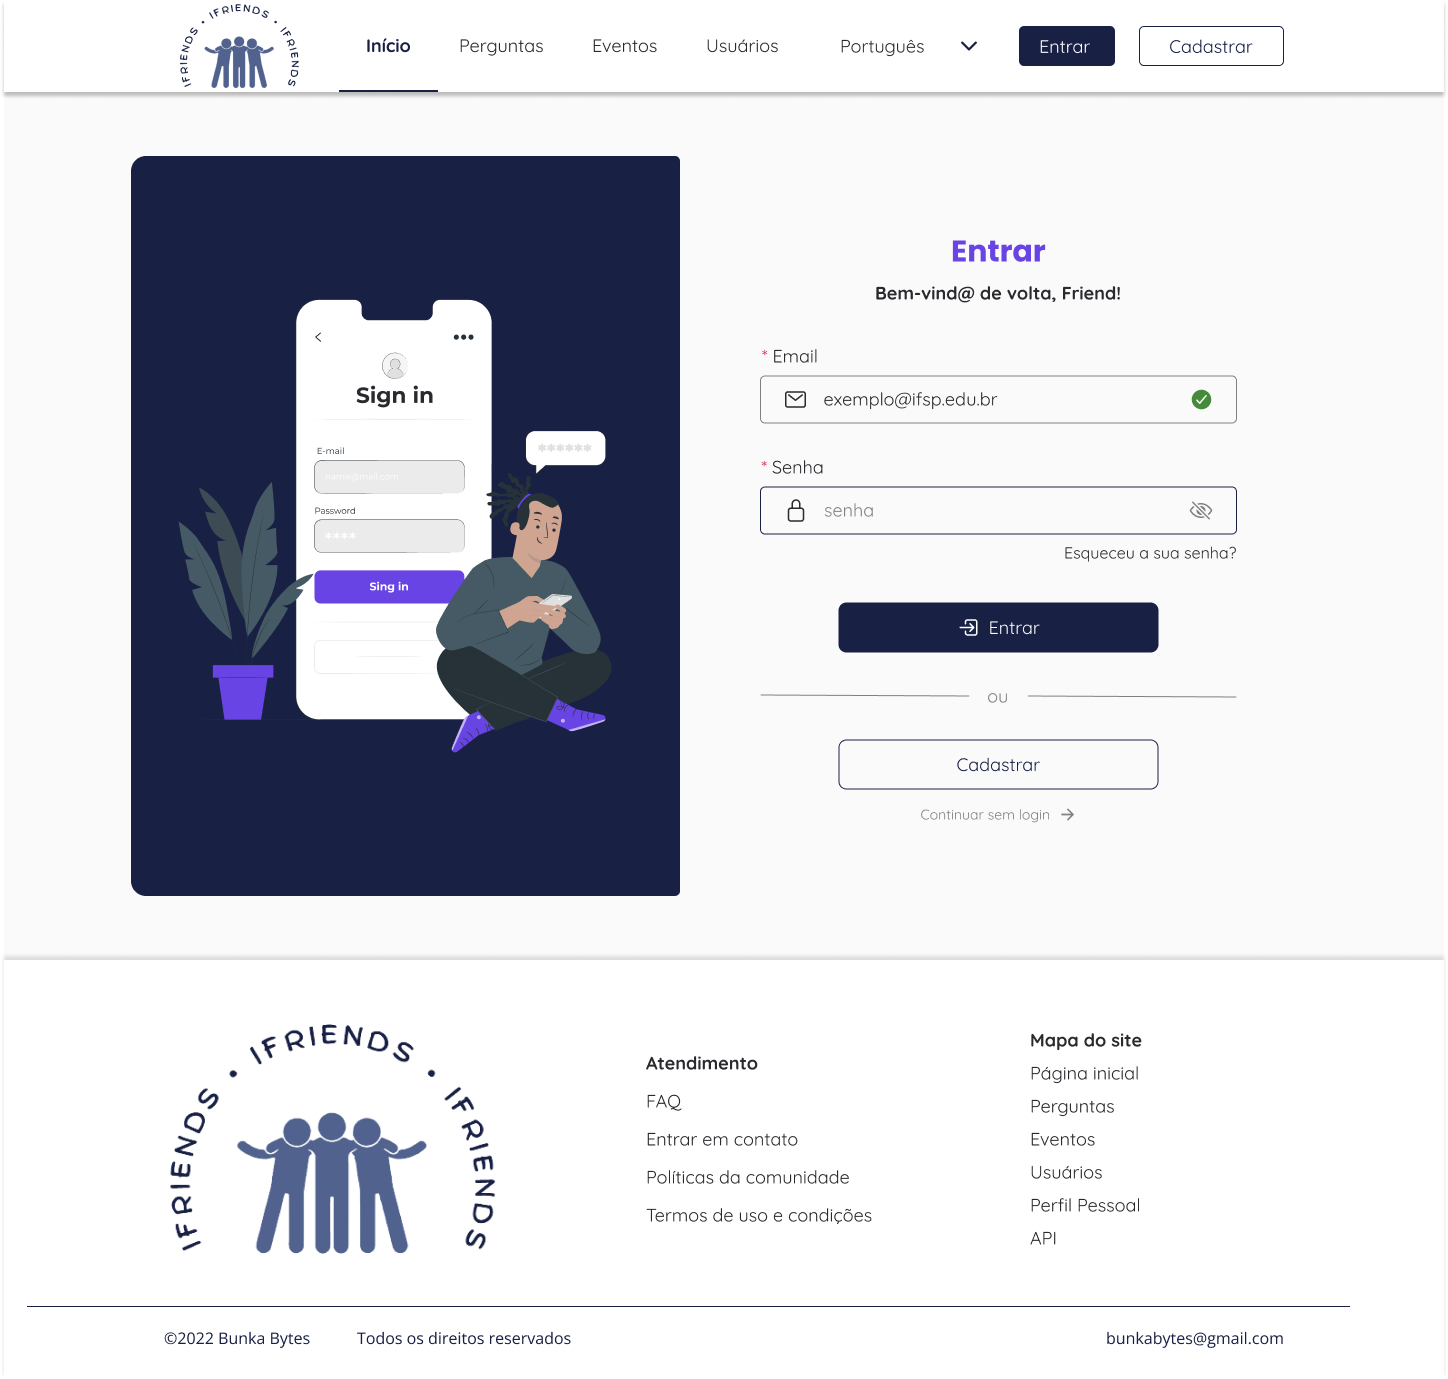
\includegraphics[width=1\textwidth]{anexos/Imagens_Prototipo/intro/login.png}
\fonte{Os autores.}
\end{figure}
\FloatBarrier

A \autoref{sl_perguntas} representa a página de perguntas, nela o \gls{friend} pode navegar por meio do menu superior ou através do filtro de categorias. 

\begin{figure}[htb]
\centering
\caption{\label{sl_perguntas} Página de perguntas}
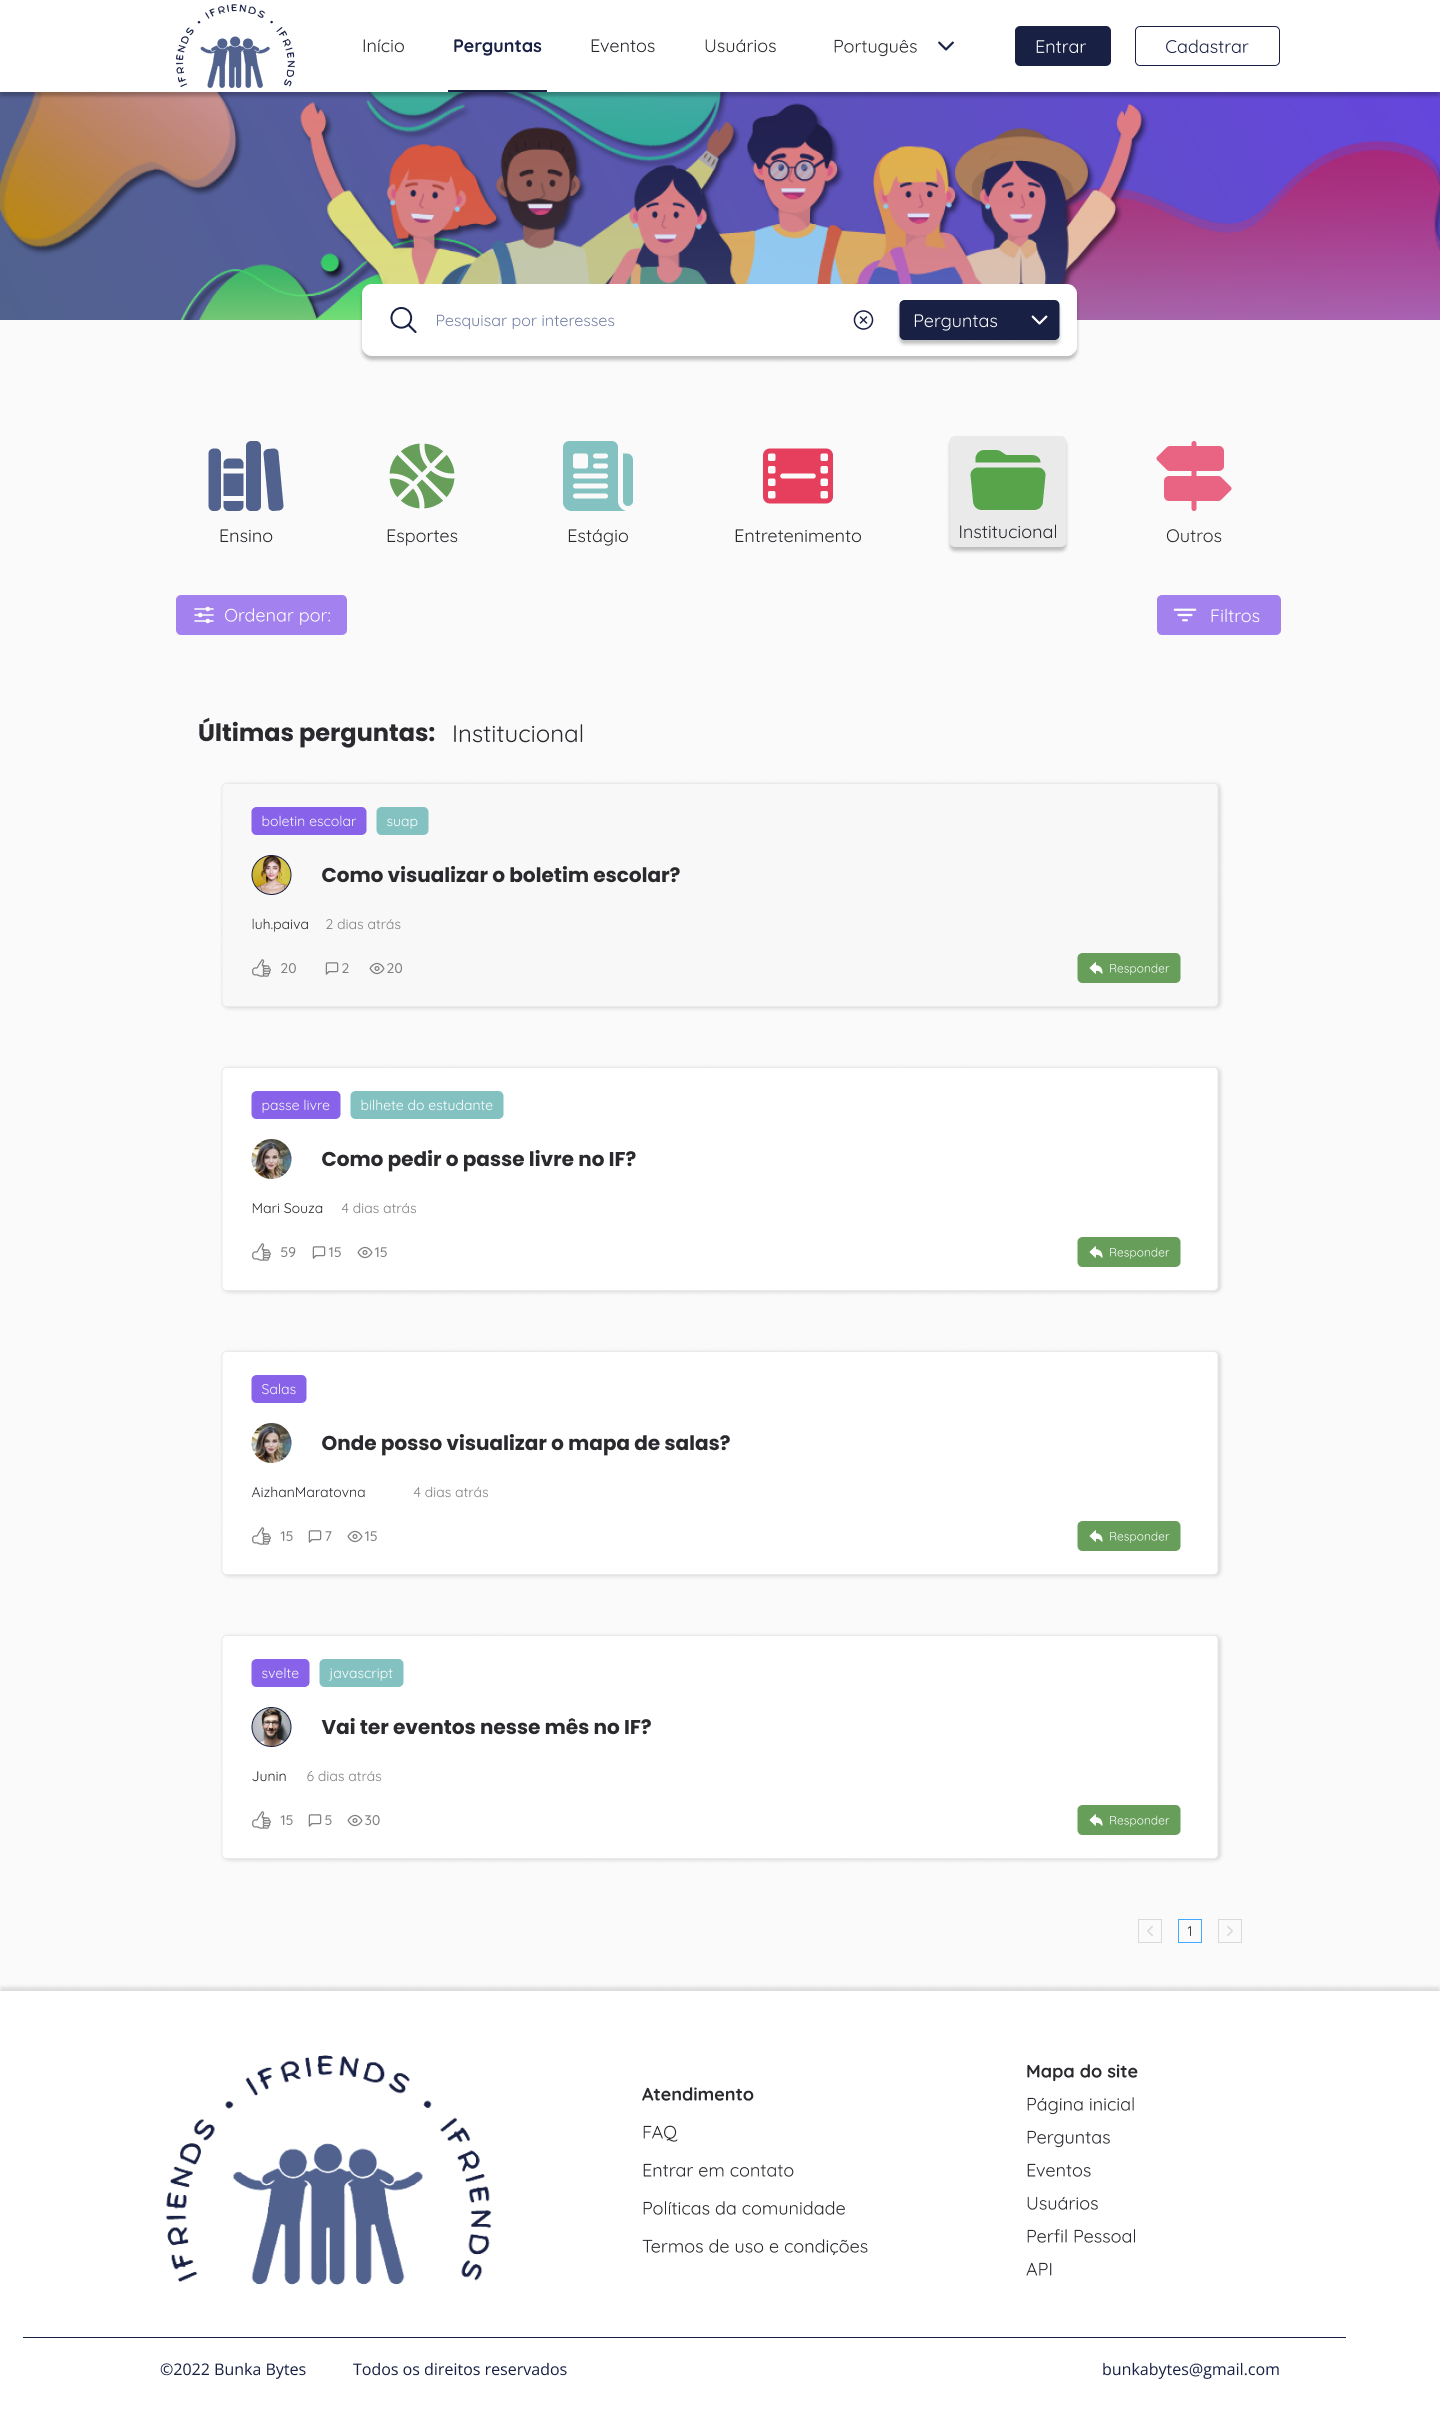
\includegraphics[width=0.8\textwidth]{anexos/Imagens_Prototipo/sem_login/perguntas.png}
\fonte{Os autores.}
\end{figure}
\FloatBarrier

A \autoref{sl_detalhes_pergunta} representa a página de detalhes da pergunta, nela é possível visualizar as respostas que aquela pergunta recebeu.

\begin{figure}[htb]
\centering
\caption{\label{sl_detalhes_pergunta} Página de detalhes da pergunta}
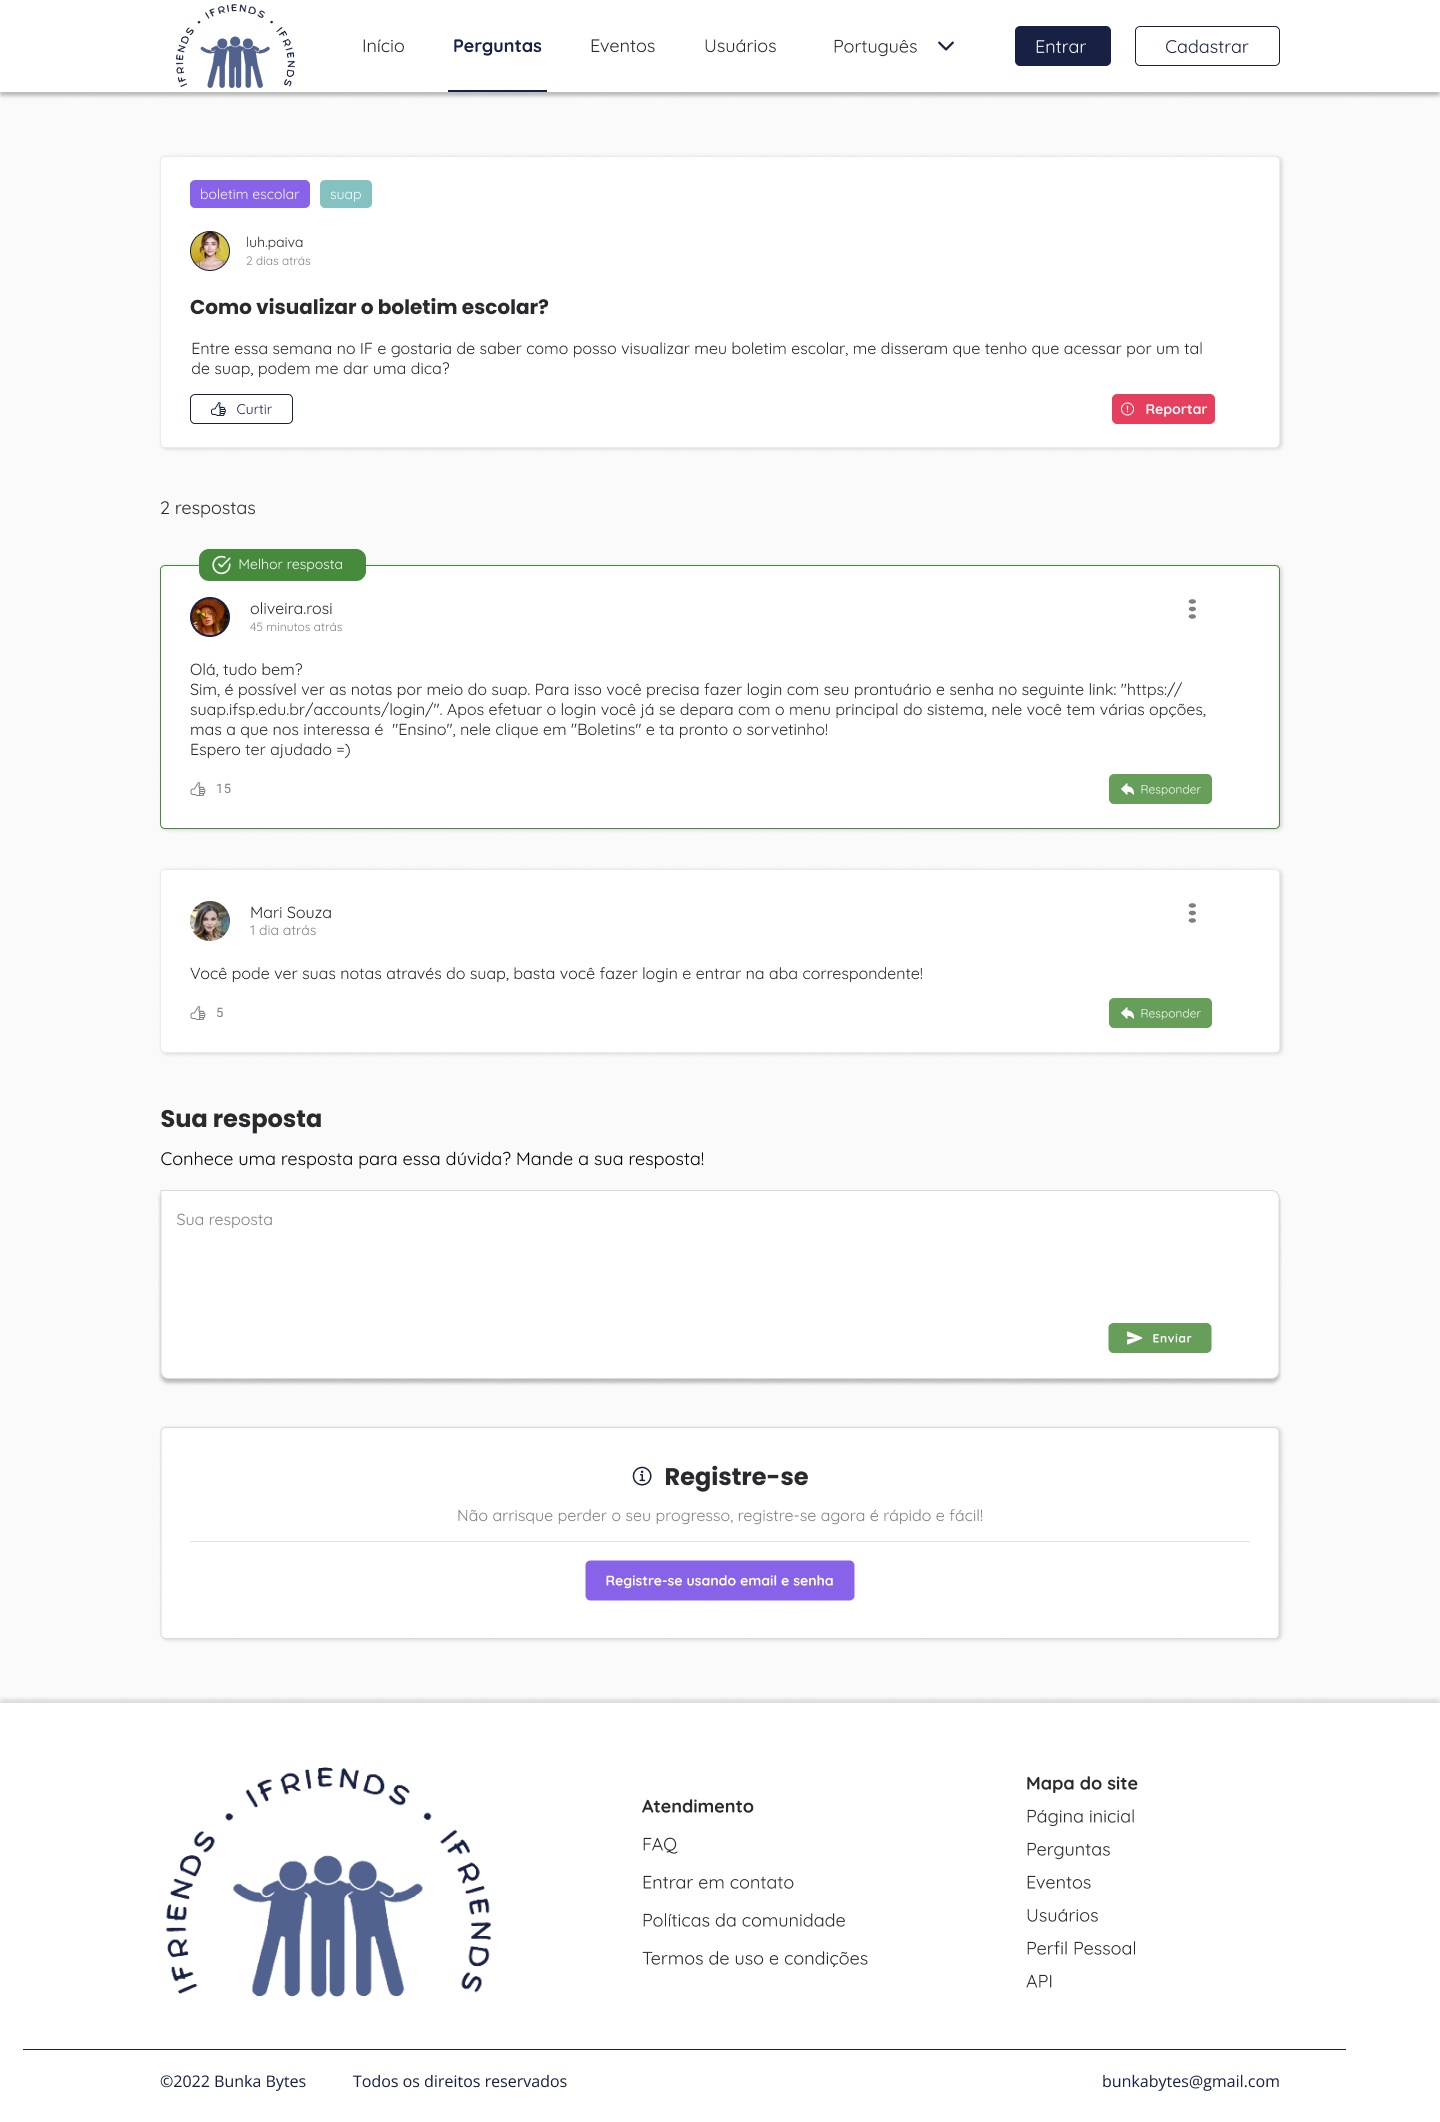
\includegraphics[width=0.8\textwidth]{anexos/Imagens_Prototipo/sem_login/pergunta_respostas.png}
\fonte{Os autores.}
\end{figure}
\FloatBarrier

A \autoref{sl_detalhes_pergunta-erro} representa um erro gerado quando o \gls{friend} tenta responder à pergunta no modo visitante, dessa forma, são apresentadas as opções de fazer \textit{login} ou fazer cadastro. 

\begin{figure}[htb]
\centering
\caption{\label{sl_detalhes_pergunta-erro} Página de detalhes da pergunta com erro}
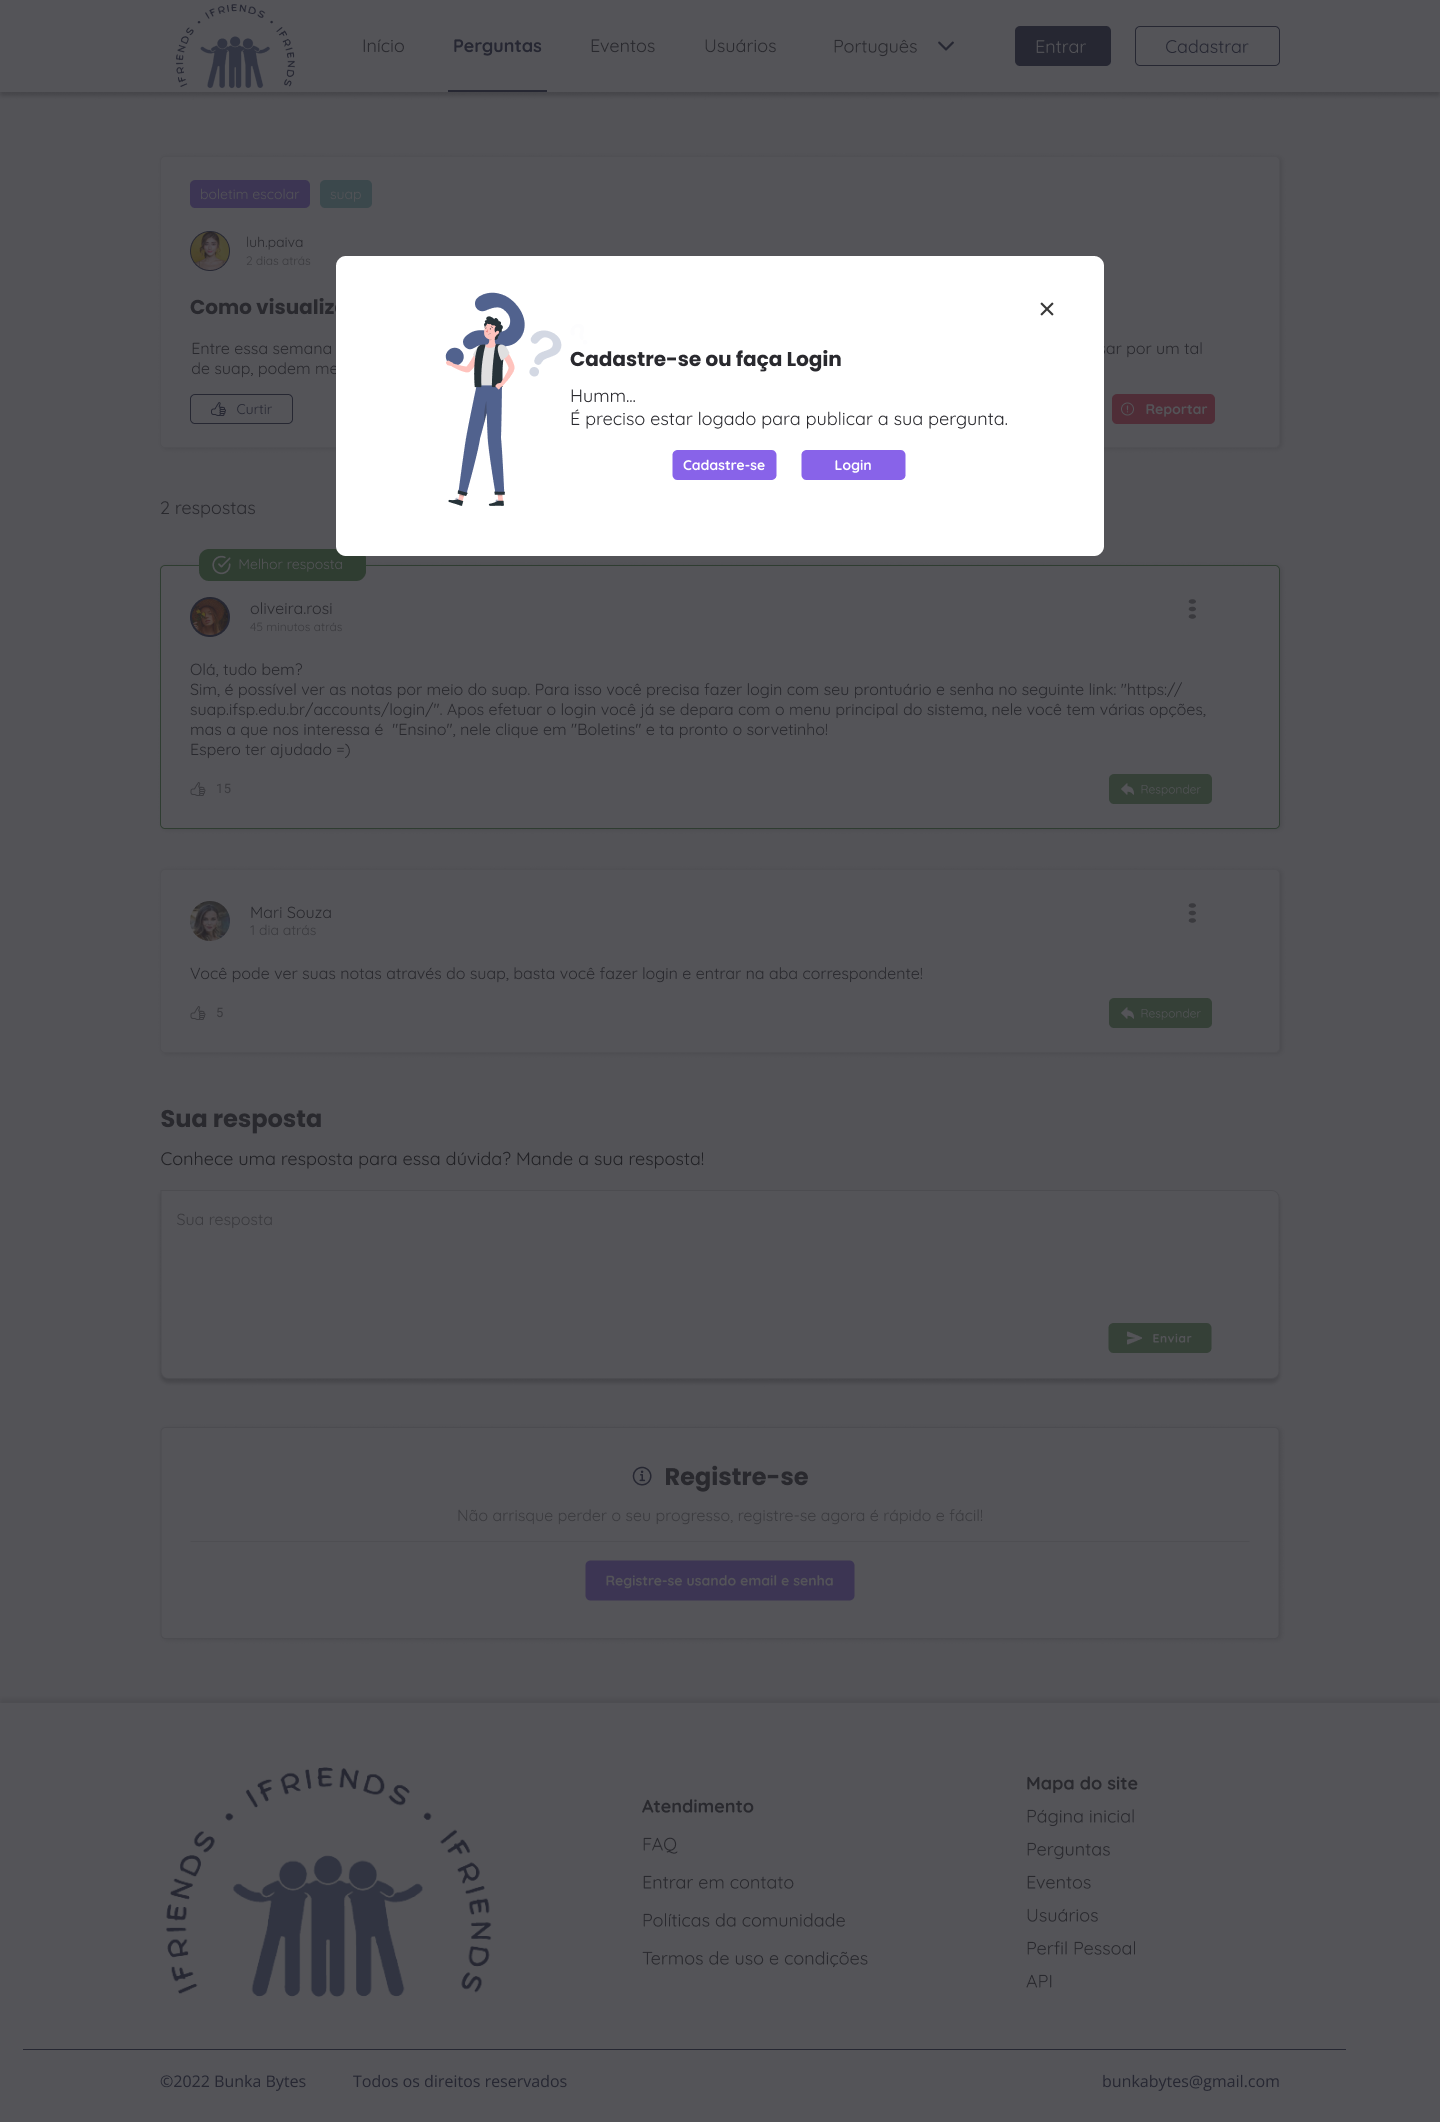
\includegraphics[width=0.8\textwidth]{anexos/Imagens_Prototipo/sem_login/pergunta_respostas-erro.png}
\fonte{Os autores.}
\end{figure}
\FloatBarrier

A \autoref{sl_eventos} representa a página de eventos, nela o \gls{friend} pode navegar por meio do menu superior ou através do filtro de categorias. 

\begin{figure}[htb]
\centering
\caption{\label{sl_eventos} Página de eventos}
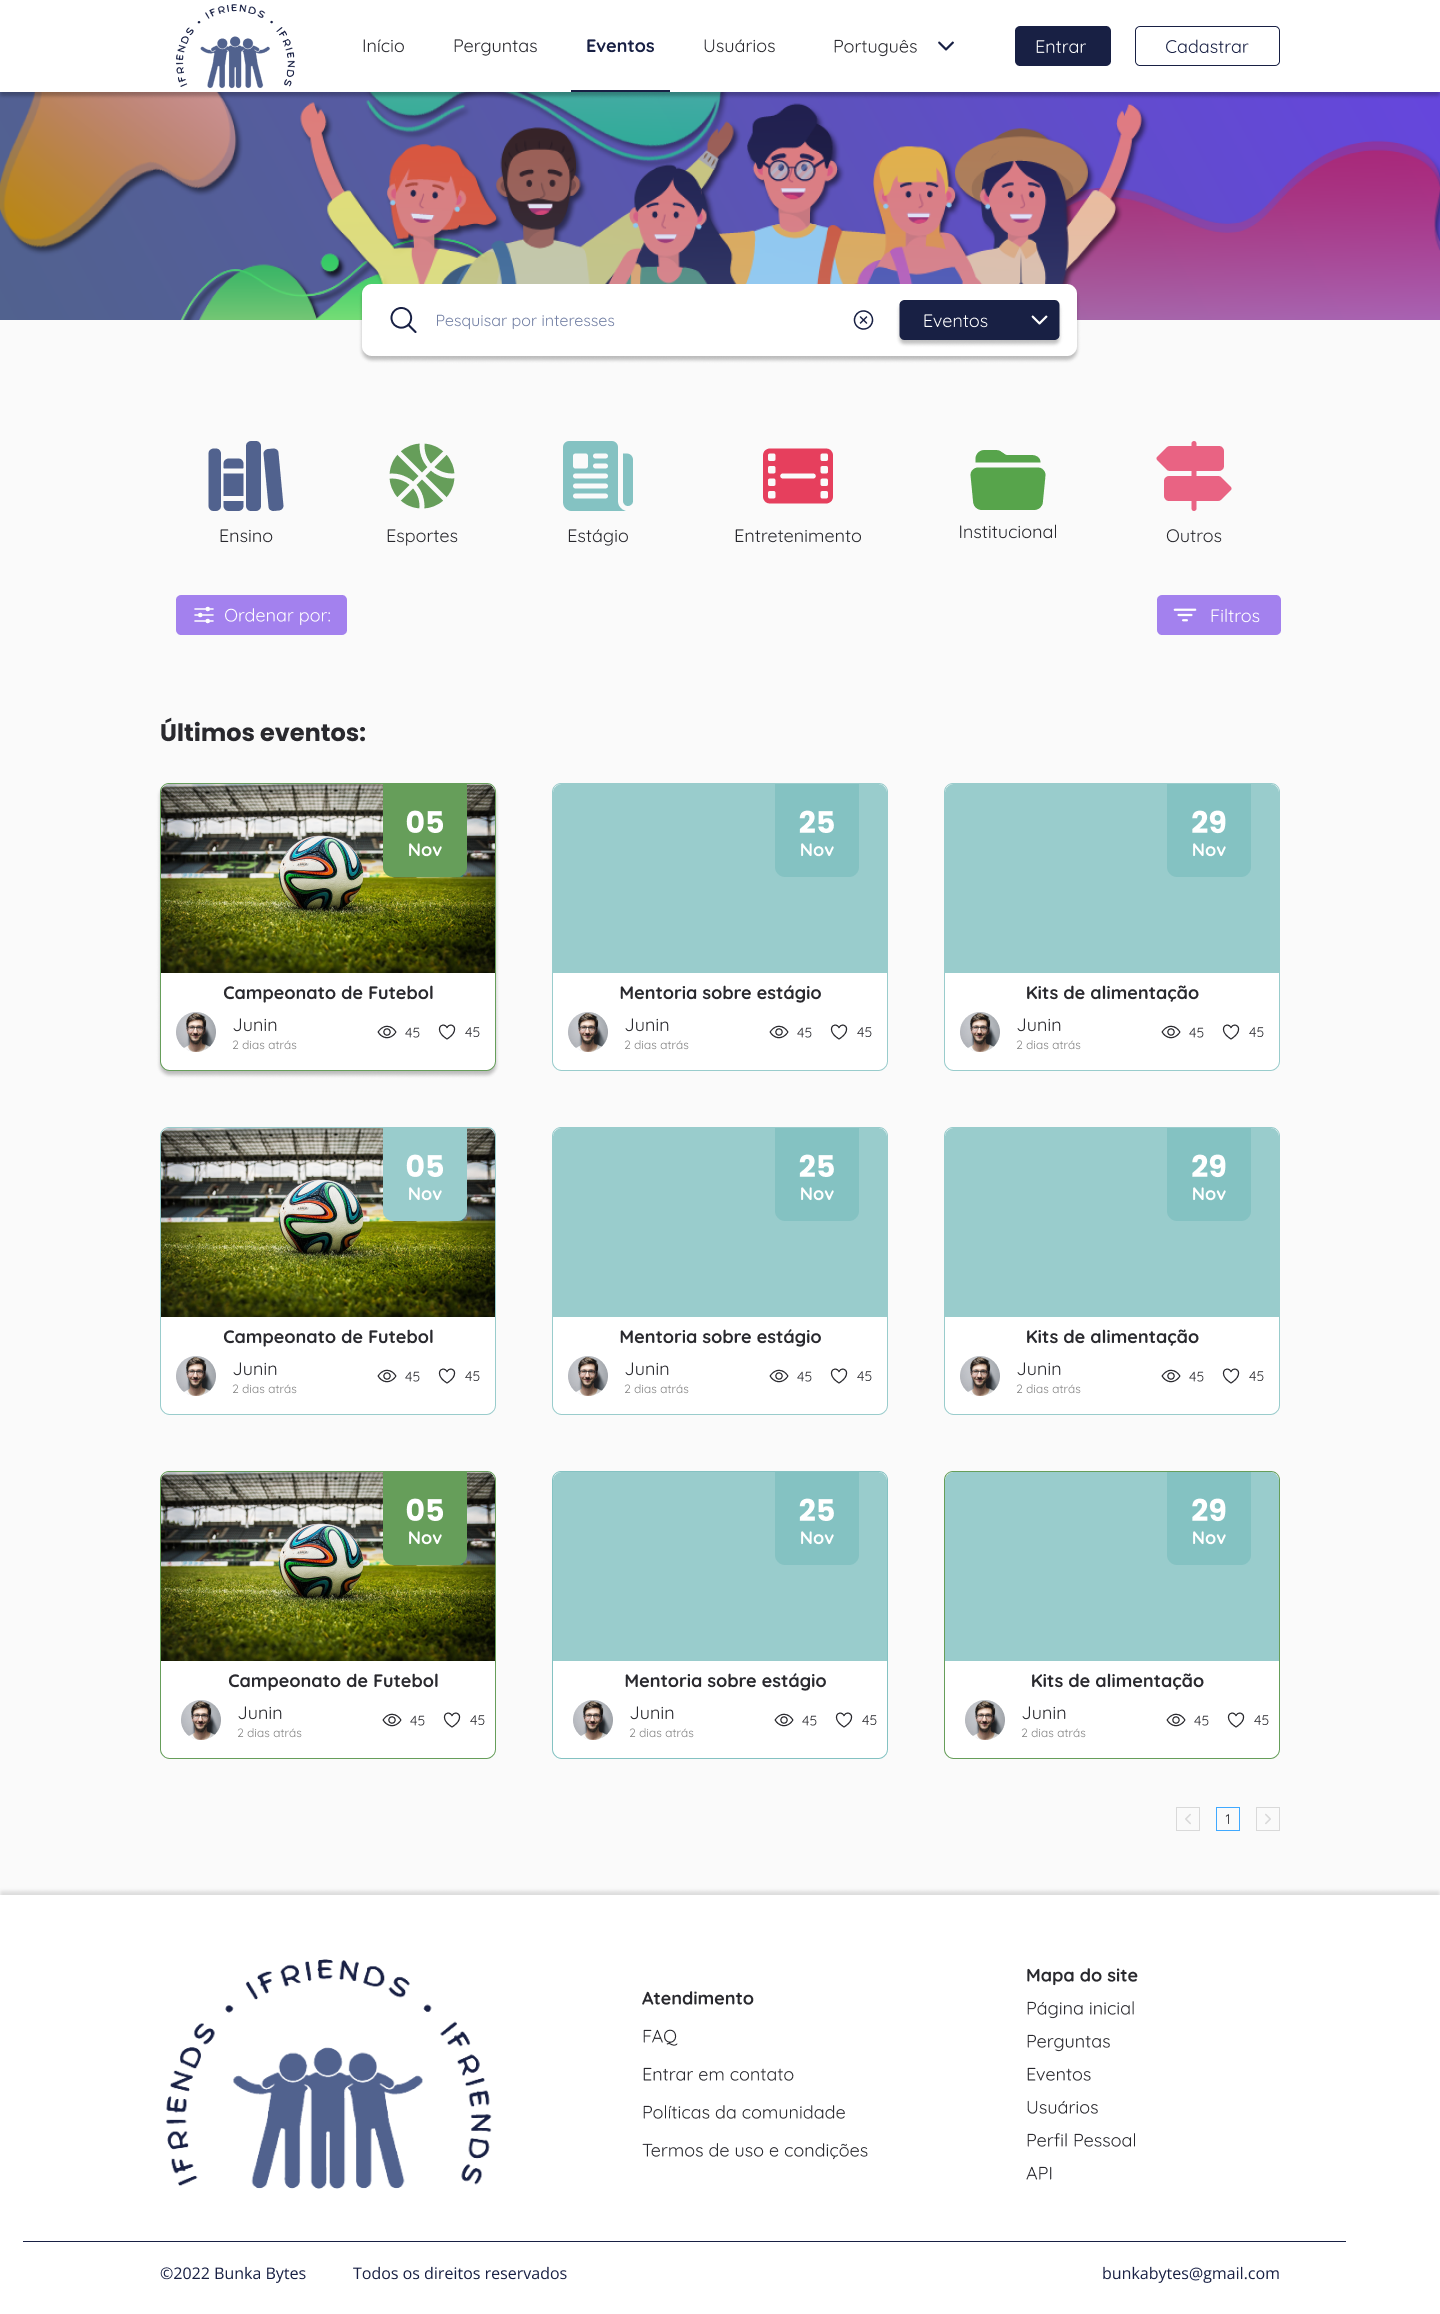
\includegraphics[width=1\textwidth]{anexos/Imagens_Prototipo/sem_login/eventos.png}
\fonte{Os autores.}
\end{figure}
\FloatBarrier

A \autoref{sl_usuarios} representa a página de usuários.

\begin{figure}[htb]
\centering
\caption{\label{sl_usuarios} Página de usuários}
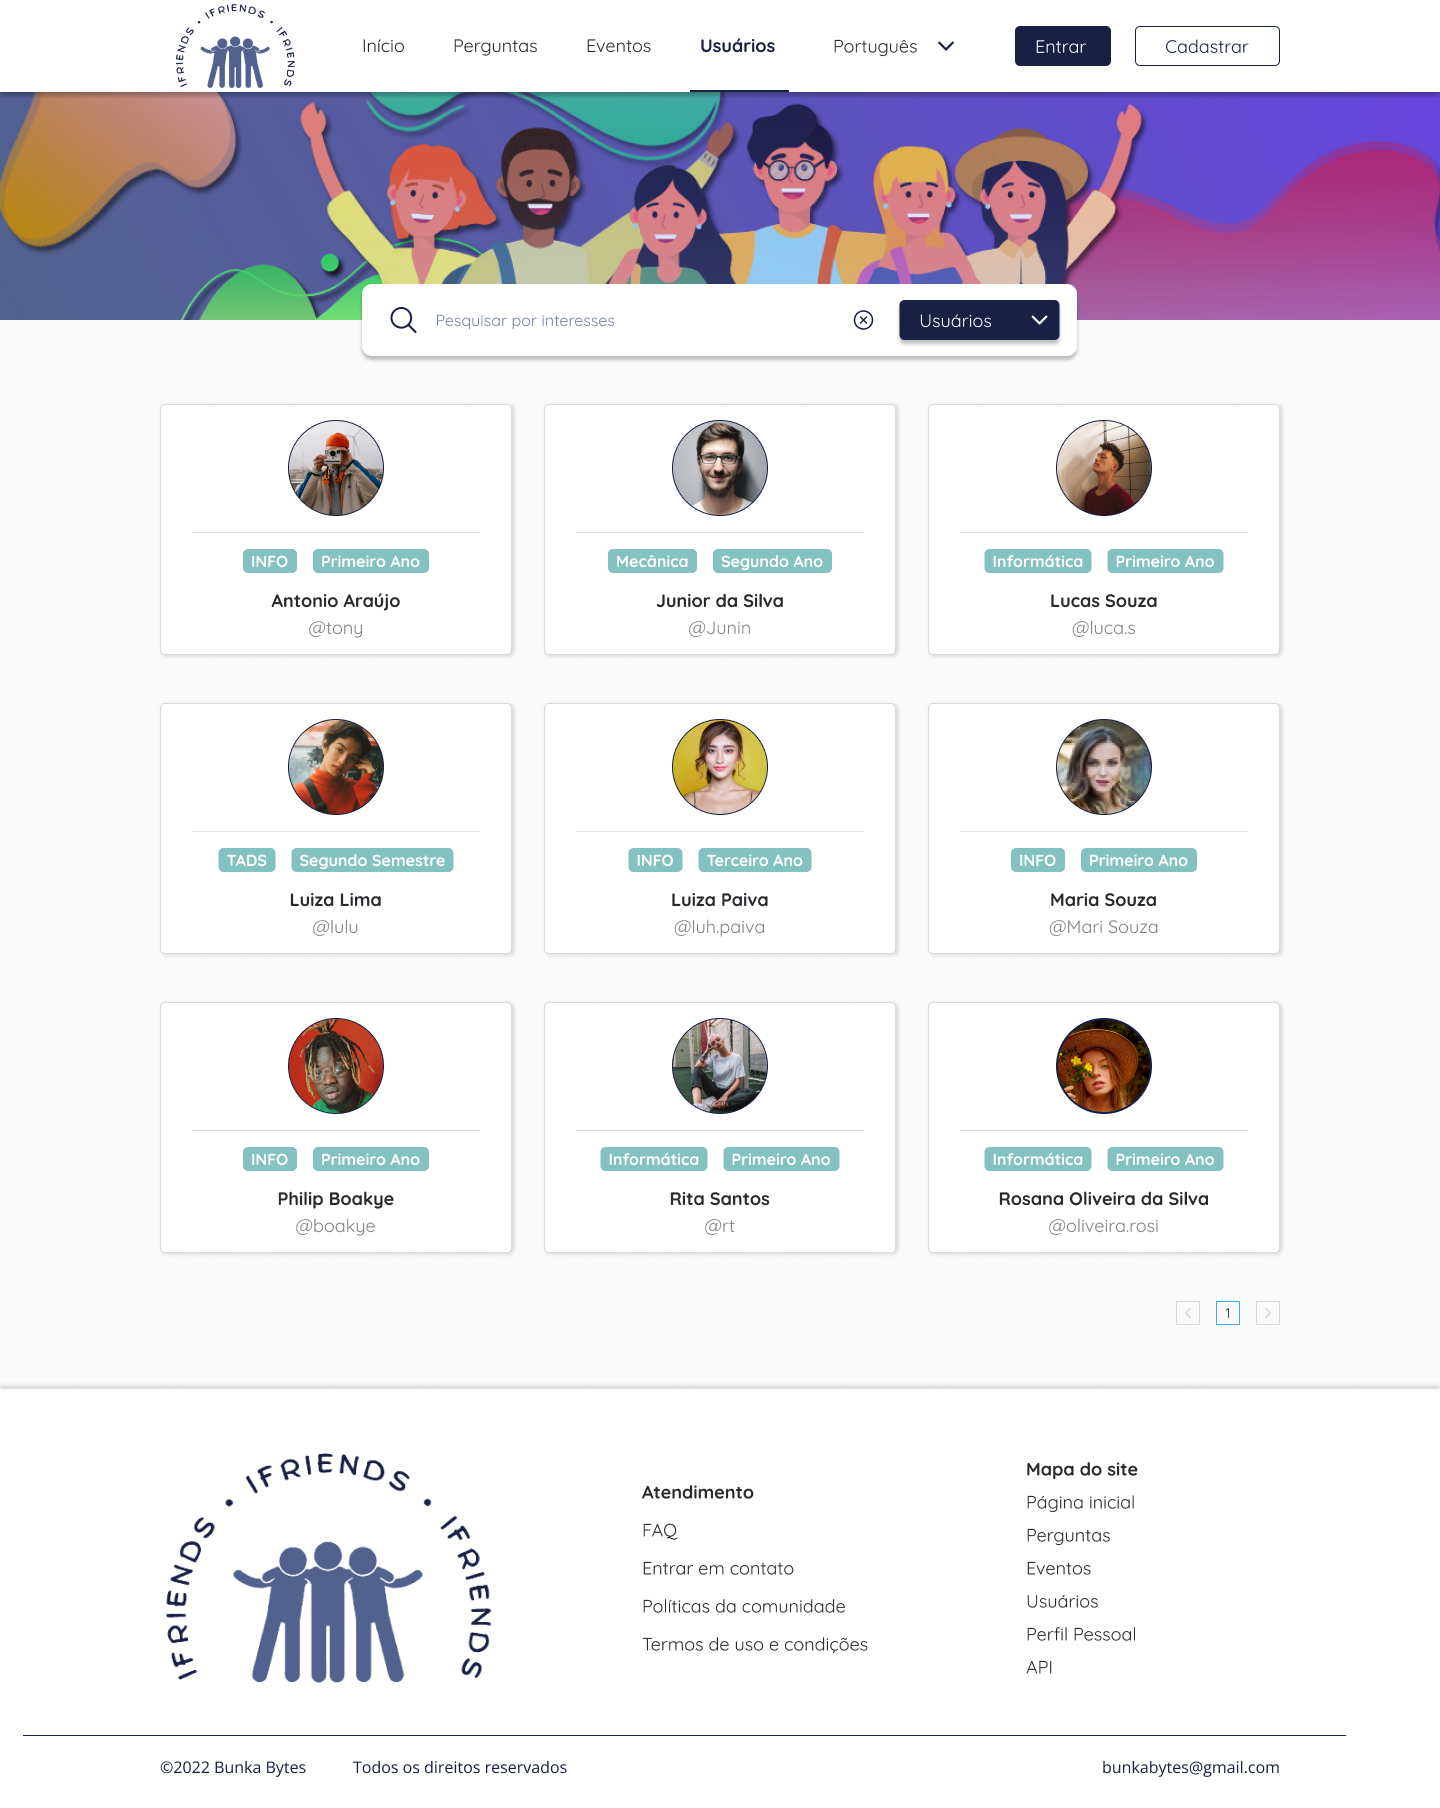
\includegraphics[width=1\textwidth]{anexos/Imagens_Prototipo/sem_login/usuarios.png}
\fonte{Os autores.}
\end{figure}
\FloatBarrier

%--------------------------------------------------------------
\section{Friend com login}
%--------------------------------------------------------------
Já para o \gls{friend} \textit{logado} no sistema, não há restrições de funcionalidades, então desde que as use com responsabilidade e da forma certa, a aplicação cumprirá o que foi proposto.

Por tanto, a \autoref{cl_perguntas} apresenta a página de perguntas, repare que diferentemente da visão do \gls{friend} sem \textit{login} agora foi inserido o ícone de perfil do usuário, no qual se encontra a internacionalização, configurações do perfil e também a opção de sair.

\begin{figure}[htb]
\centering
\caption{\label{cl_perguntas} Página de perguntas}
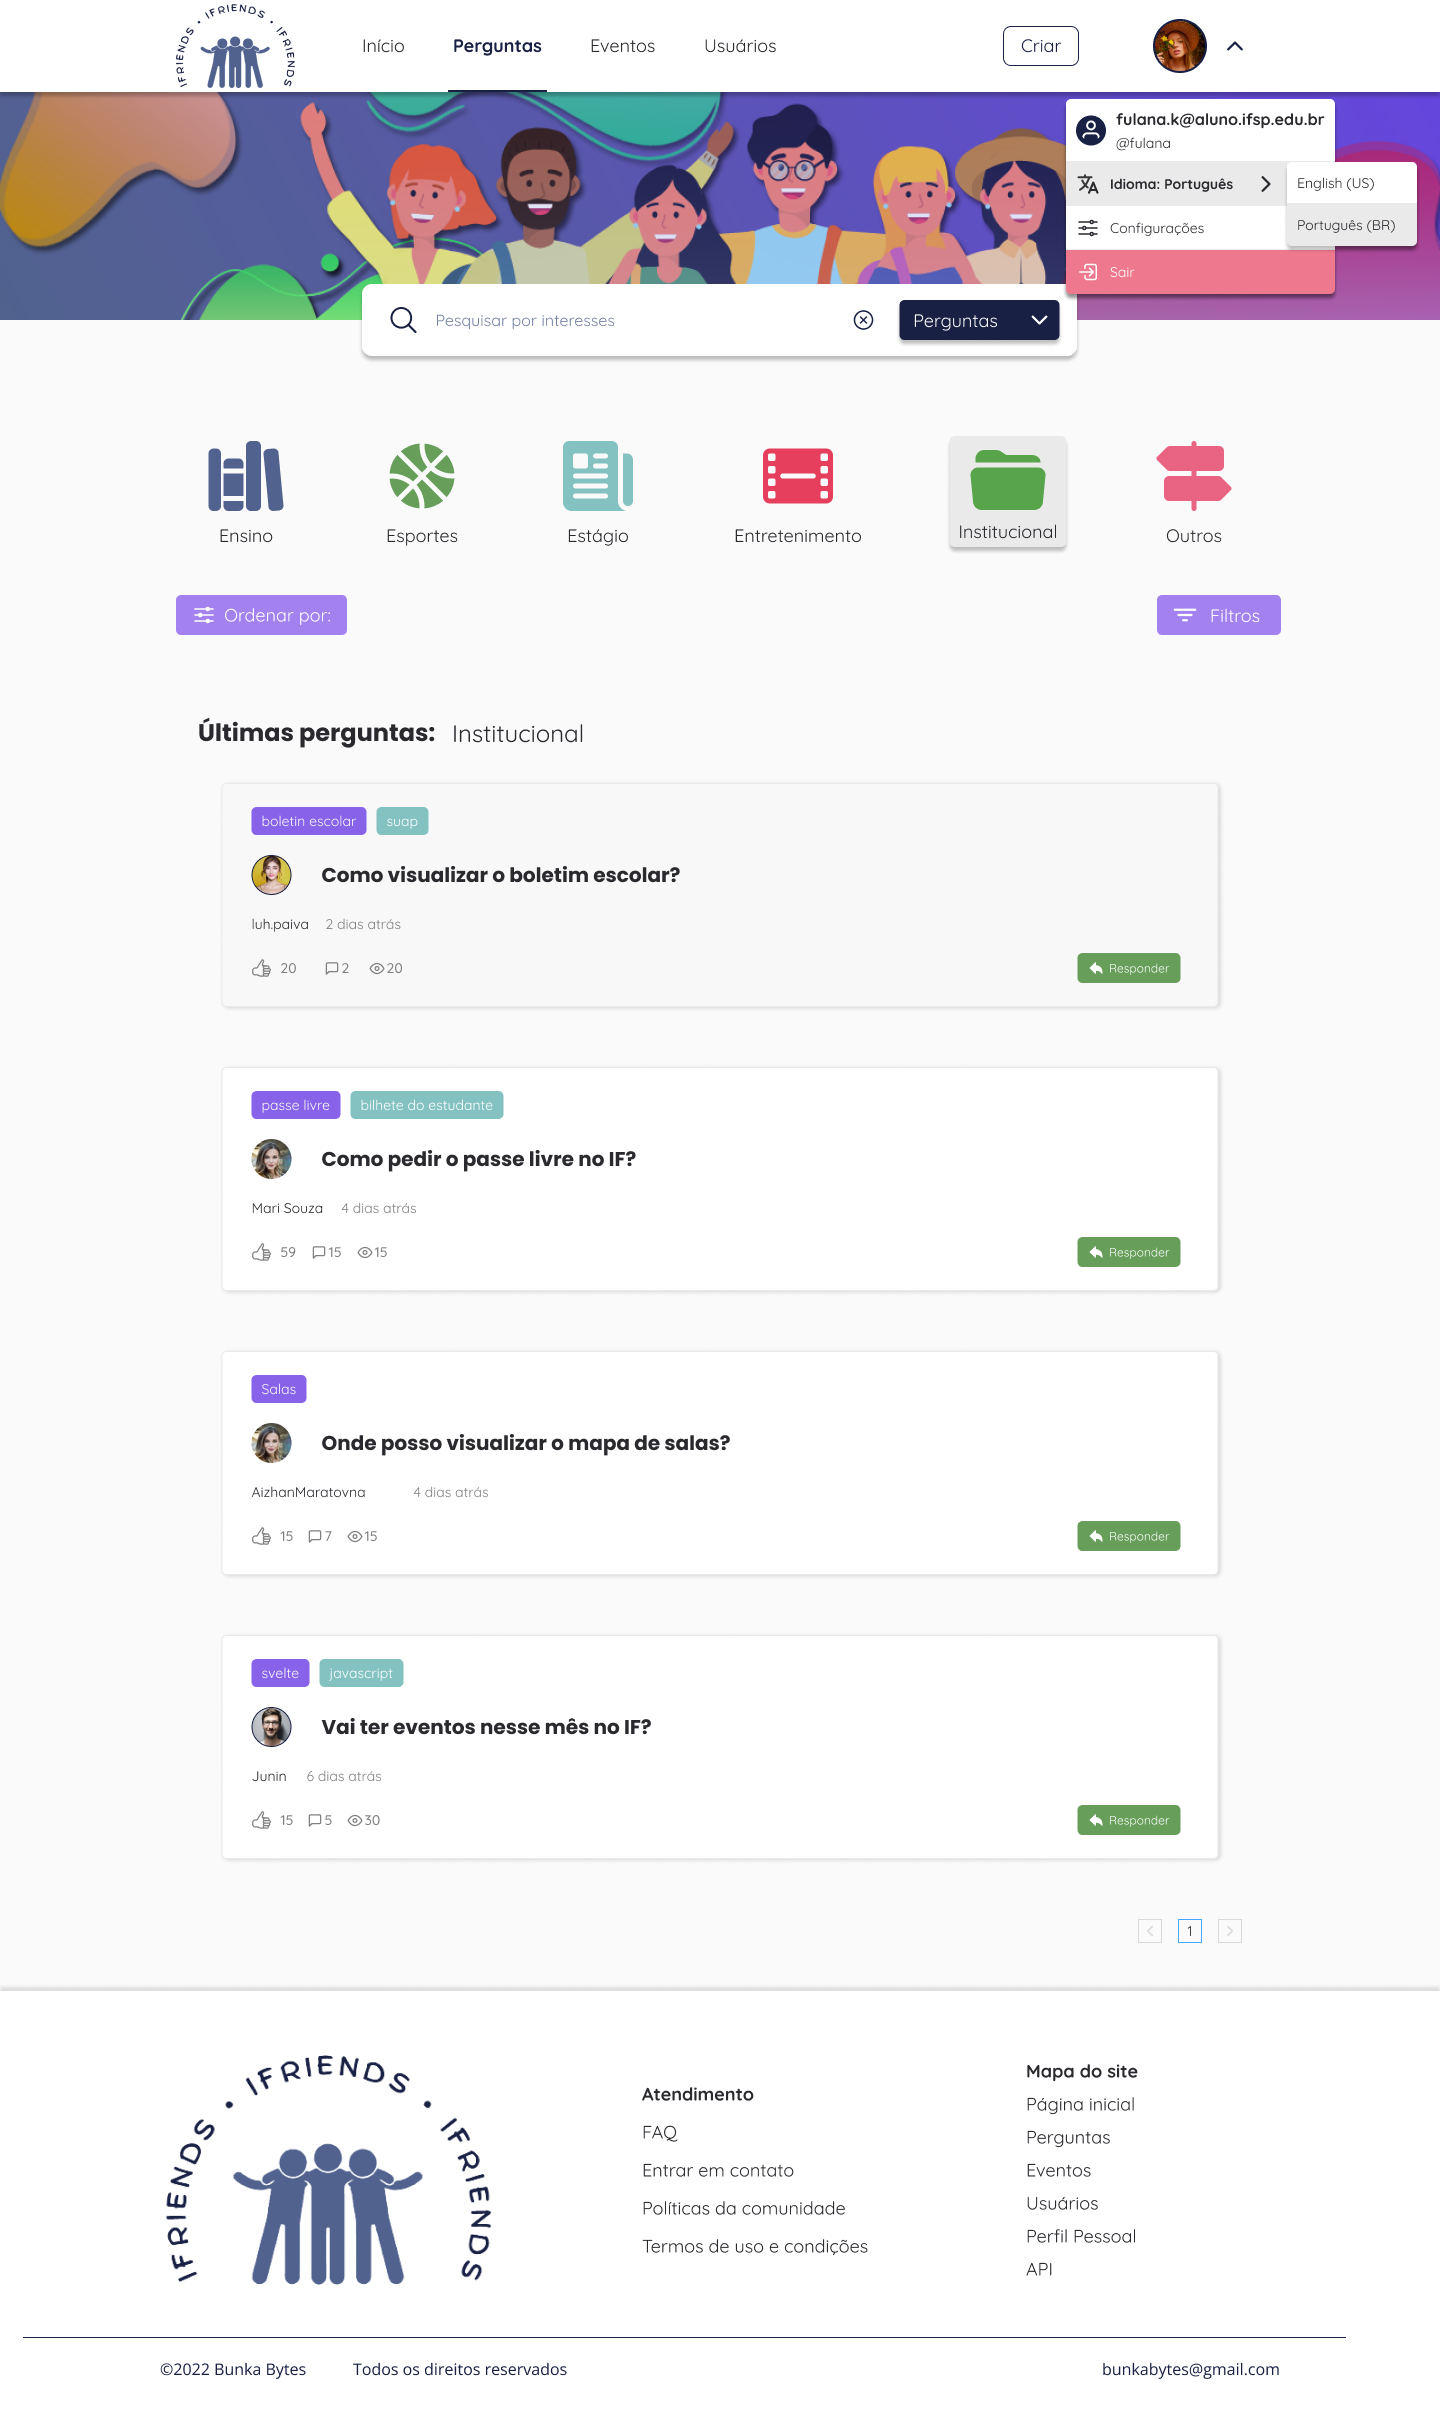
\includegraphics[width=0.8\textwidth]{anexos/Imagens_Prototipo/com_login/perguntas.png}
\fonte{Os autores.}
\end{figure}
\FloatBarrier

Quando o \gls{friend} clica em uma pergunta ou em ``Responder'' ele é direcionado à página dessa pergunta como mostra a \autoref{cl_detalhes_pergunta}, nela ele pode encontrar as respostas já fornecidas por outros membros da comunidade, obter mais informações sobre a pergunta (no caso dela ter imagem), assim como também pode deixar a sua contribuição.

\begin{figure}[htb]
\centering
\caption{\label{cl_detalhes_pergunta} Página de detalhes da pergunta}
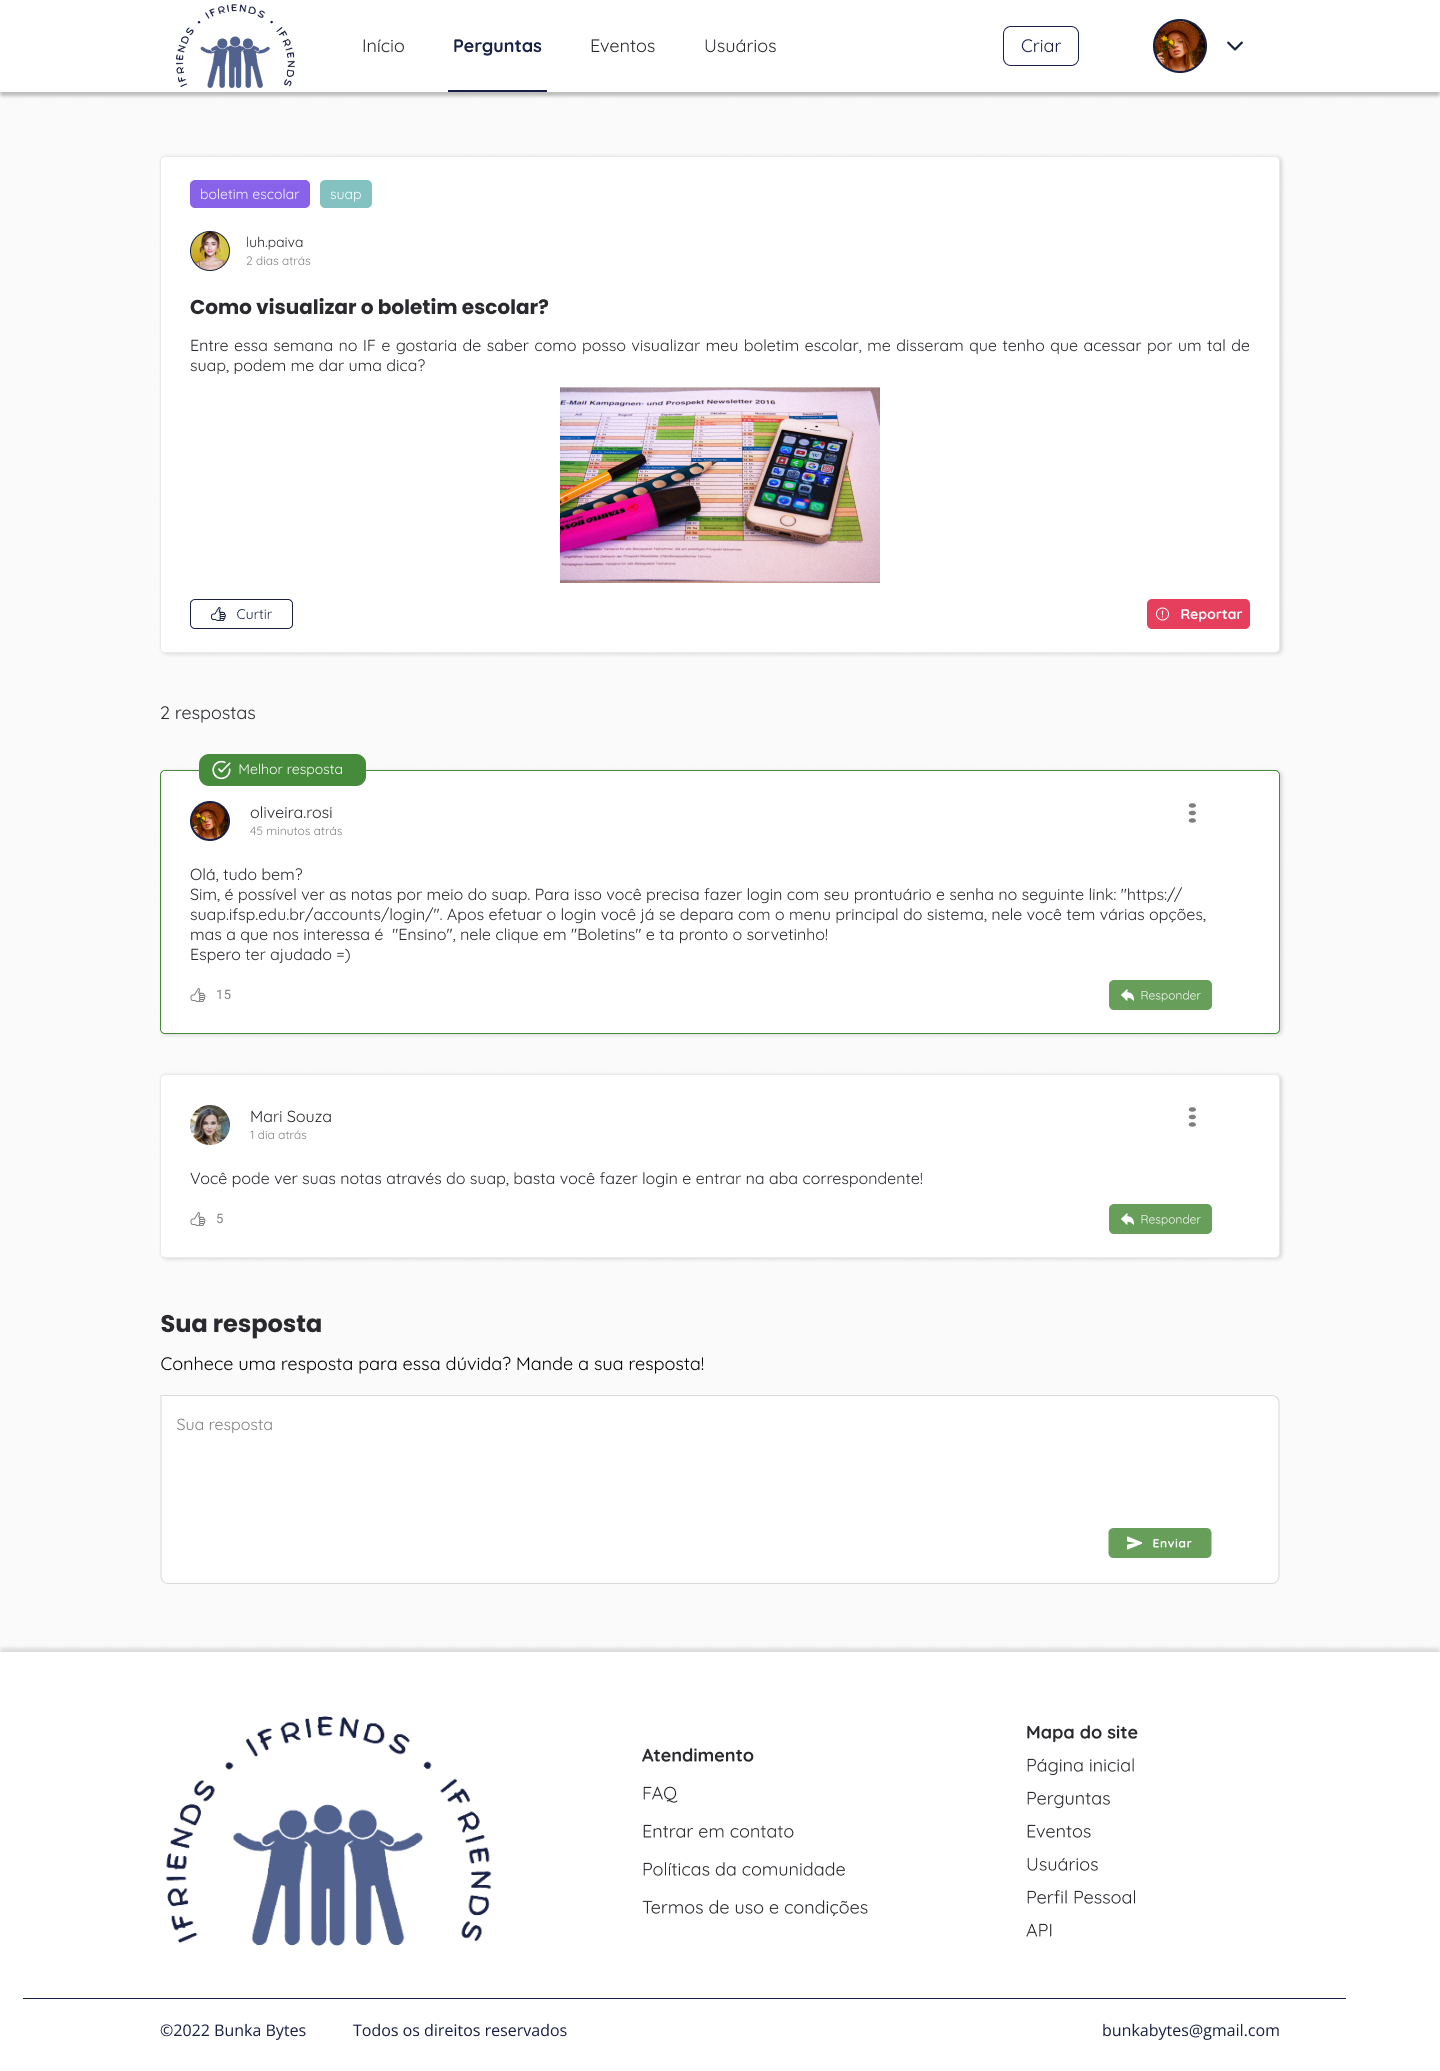
\includegraphics[width=0.8\textwidth]{anexos/Imagens_Prototipo/com_login/detalhes_perguntas.png}
\fonte{Os autores.}
\end{figure}
\FloatBarrier

Caso o \gls{friend} identifique algum comportamento inadequado ou que viole a política da comunidade, ele tem a possibilidade de reportar o ocorrido, como mostra a \autoref{cl_pergunta-reportar_respostas}.

\begin{figure}[htb]
\centering
\caption{\label{cl_pergunta-reportar_respostas} Página de reportar}
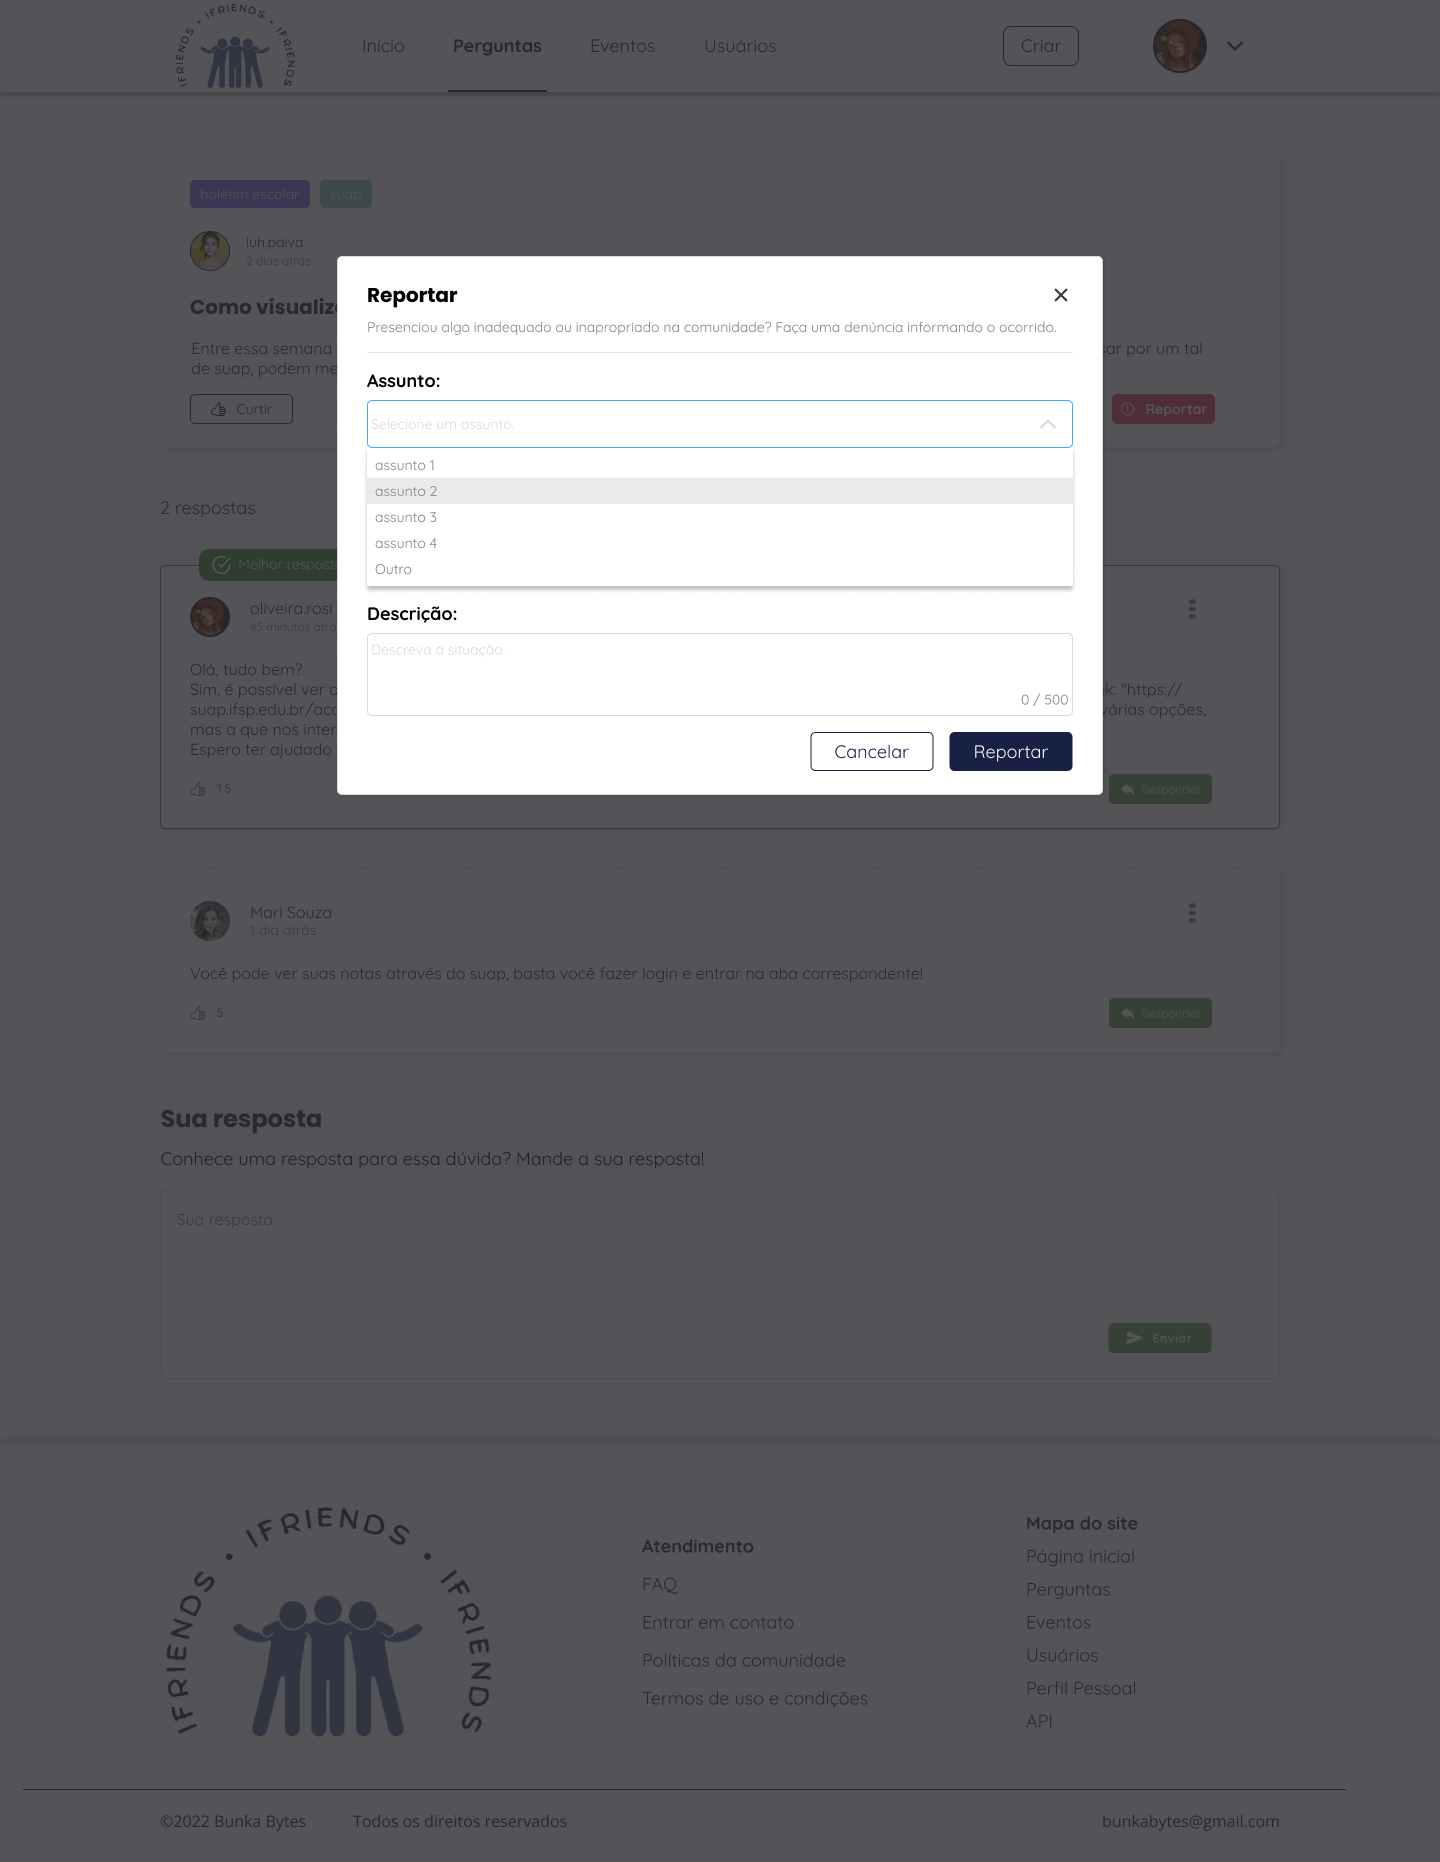
\includegraphics[width=0.8\textwidth]{anexos/Imagens_Prototipo/com_login/pergunta-reportar_respostas.png}
\fonte{Os autores.}
\end{figure}
\FloatBarrier

Já a \autoref{cadastro_perguntas} corresponde a página de cadastro de perguntas, nessa tela são apresentados todos os elementos necessários para a sua realização, assim como o manual de uma boa pergunta (\autoref{boapergunta}), elaborado com o intuito de auxiliar o \gls{friend}. 

\begin{figure}[htb]
\centering
\caption{\label{cadastro_perguntas} Página de cadastro de perguntas}
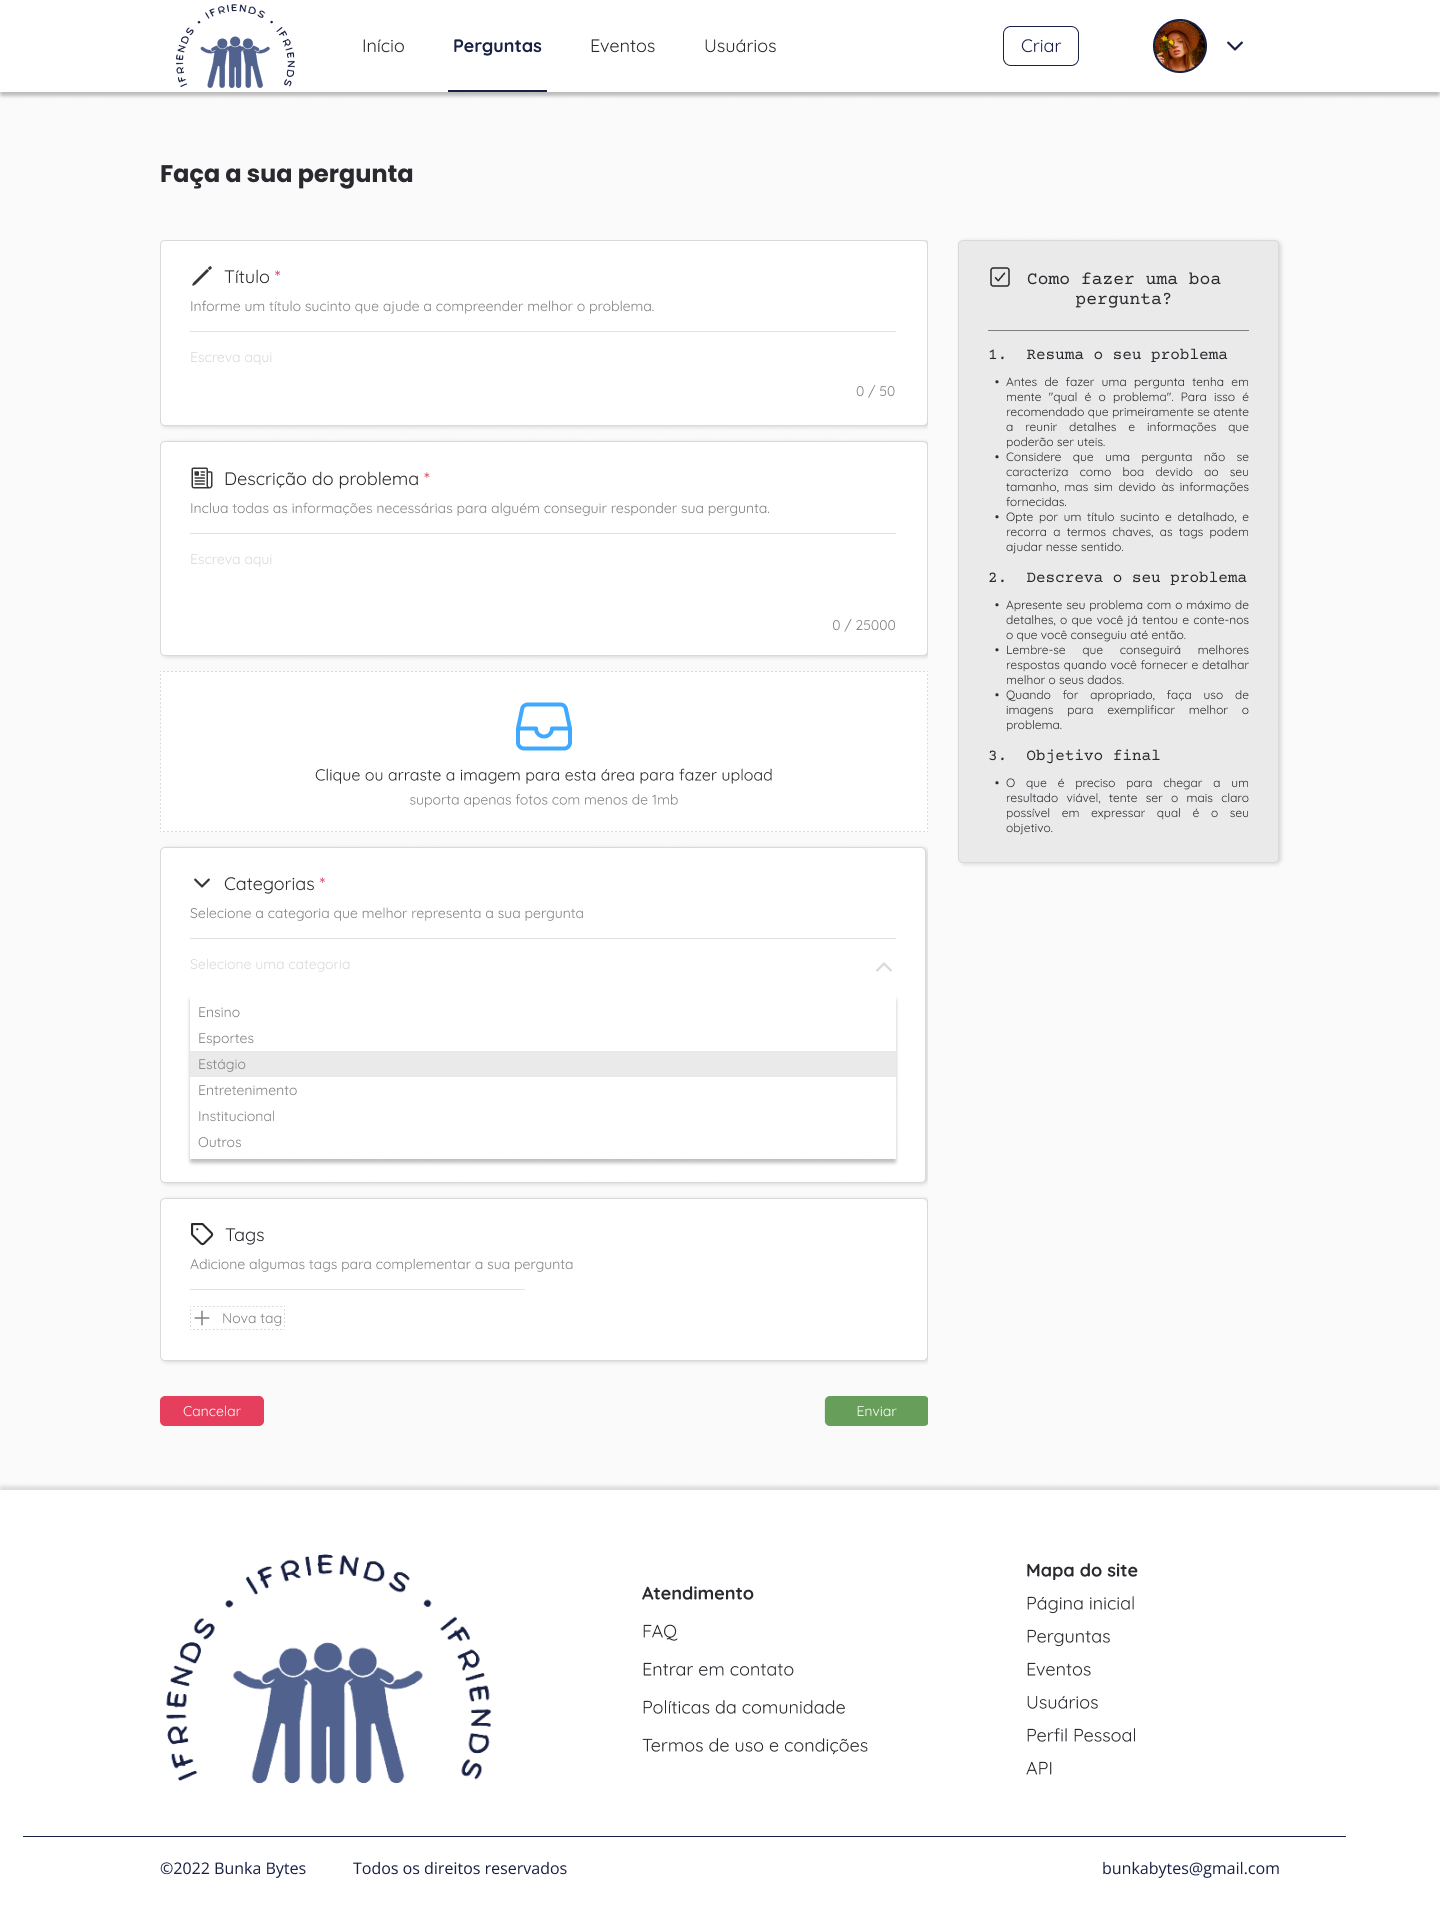
\includegraphics[width=0.8\textwidth]{anexos/Imagens_Prototipo/com_login/cadastro_perguntas.png}
\fonte{Os autores.}
\end{figure}
\FloatBarrier

A \autoref{cl_eventos} representa a página de eventos, repare que outro elemento introduzido foi o botão de ``Criar'', nele o \gls{friend} consegue facilmente ser direcionado a página de criação de um evento ou de uma pergunta.

\begin{figure}[htb]
\centering
\caption{\label{cl_eventos} Página de eventos}
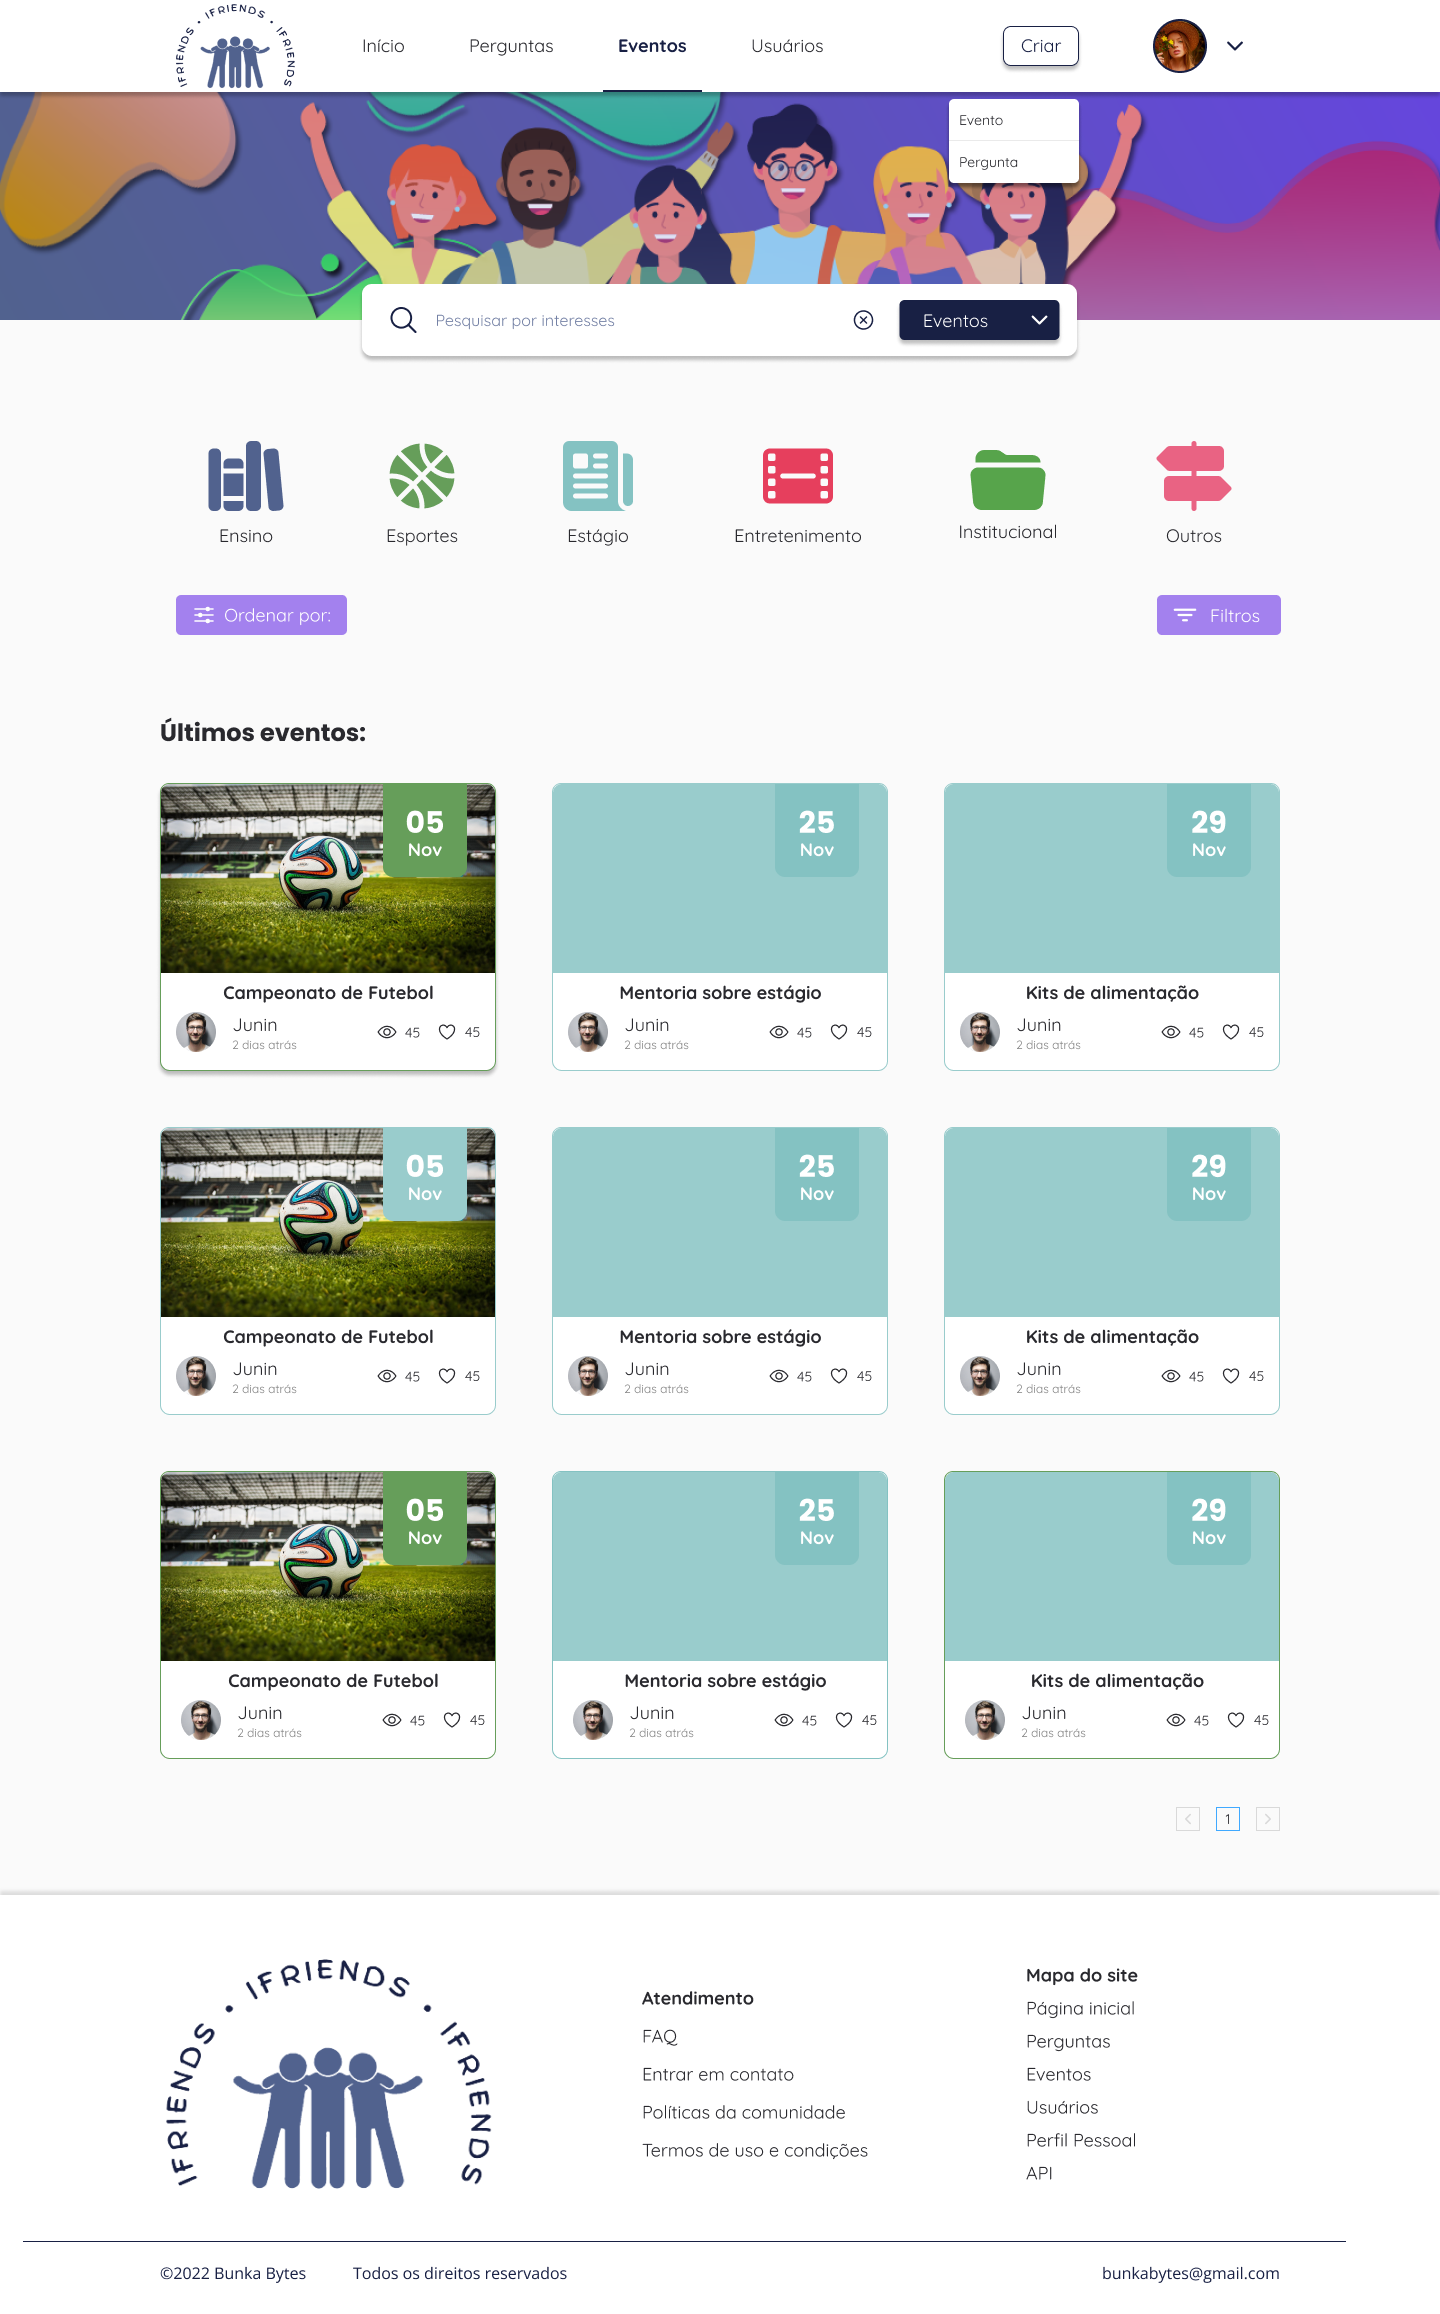
\includegraphics[width=0.8\textwidth]{anexos/Imagens_Prototipo/com_login/eventos.png}
\fonte{Os autores.}
\end{figure}
\FloatBarrier

A \autoref{cl_detalhes_evento} representa a página de detalhes do evento, nela é possível visualizar mais detalhes do evento.

\begin{figure}[htb]
\centering
\caption{\label{cl_detalhes_evento} Página de detalhes do evento}
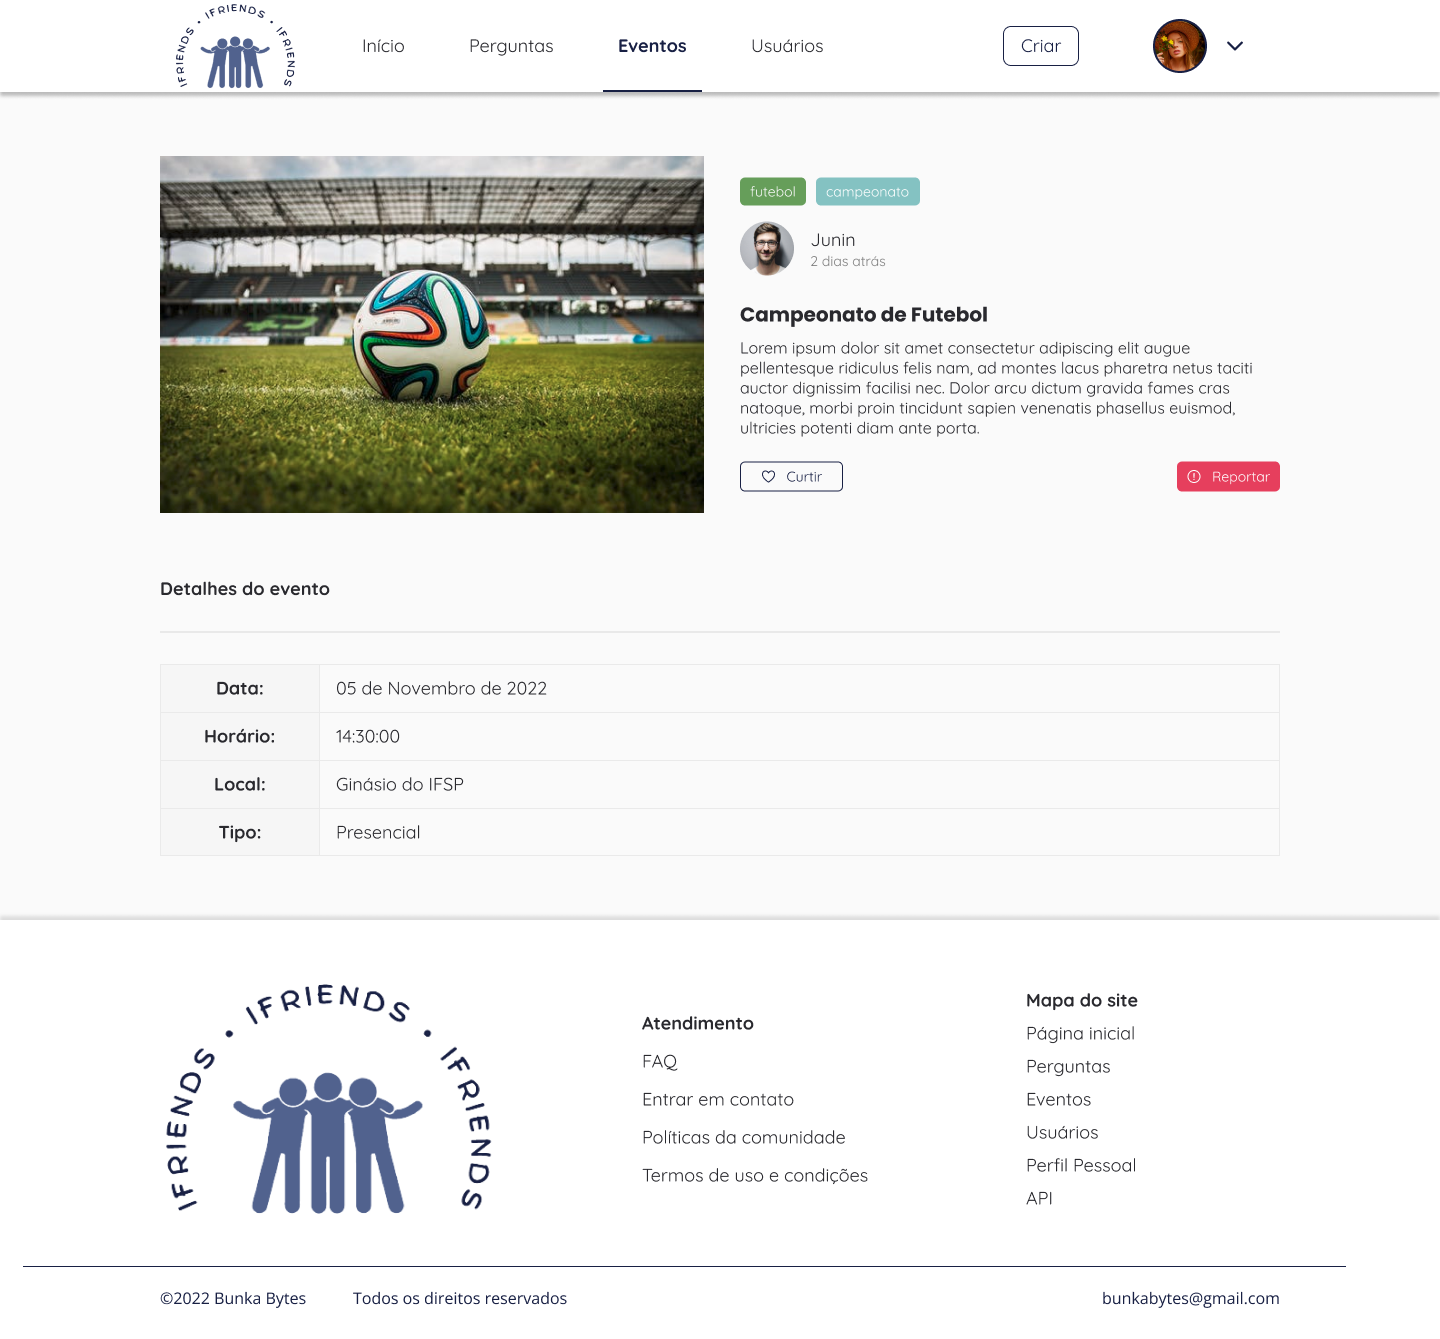
\includegraphics[width=0.8\textwidth]{anexos/Imagens_Prototipo/com_login/detalhes_eventos.png}
\fonte{Os autores.}
\end{figure}
\FloatBarrier

Já a \autoref{cadastro_evento} corresponde a página de cadastro de eventos, nessa tela são pedidos informações importantes para realizar o cadastro. 

\begin{figure}[htb]
\centering
\caption{\label{cadastro_evento} Página de cadastro de eventos}
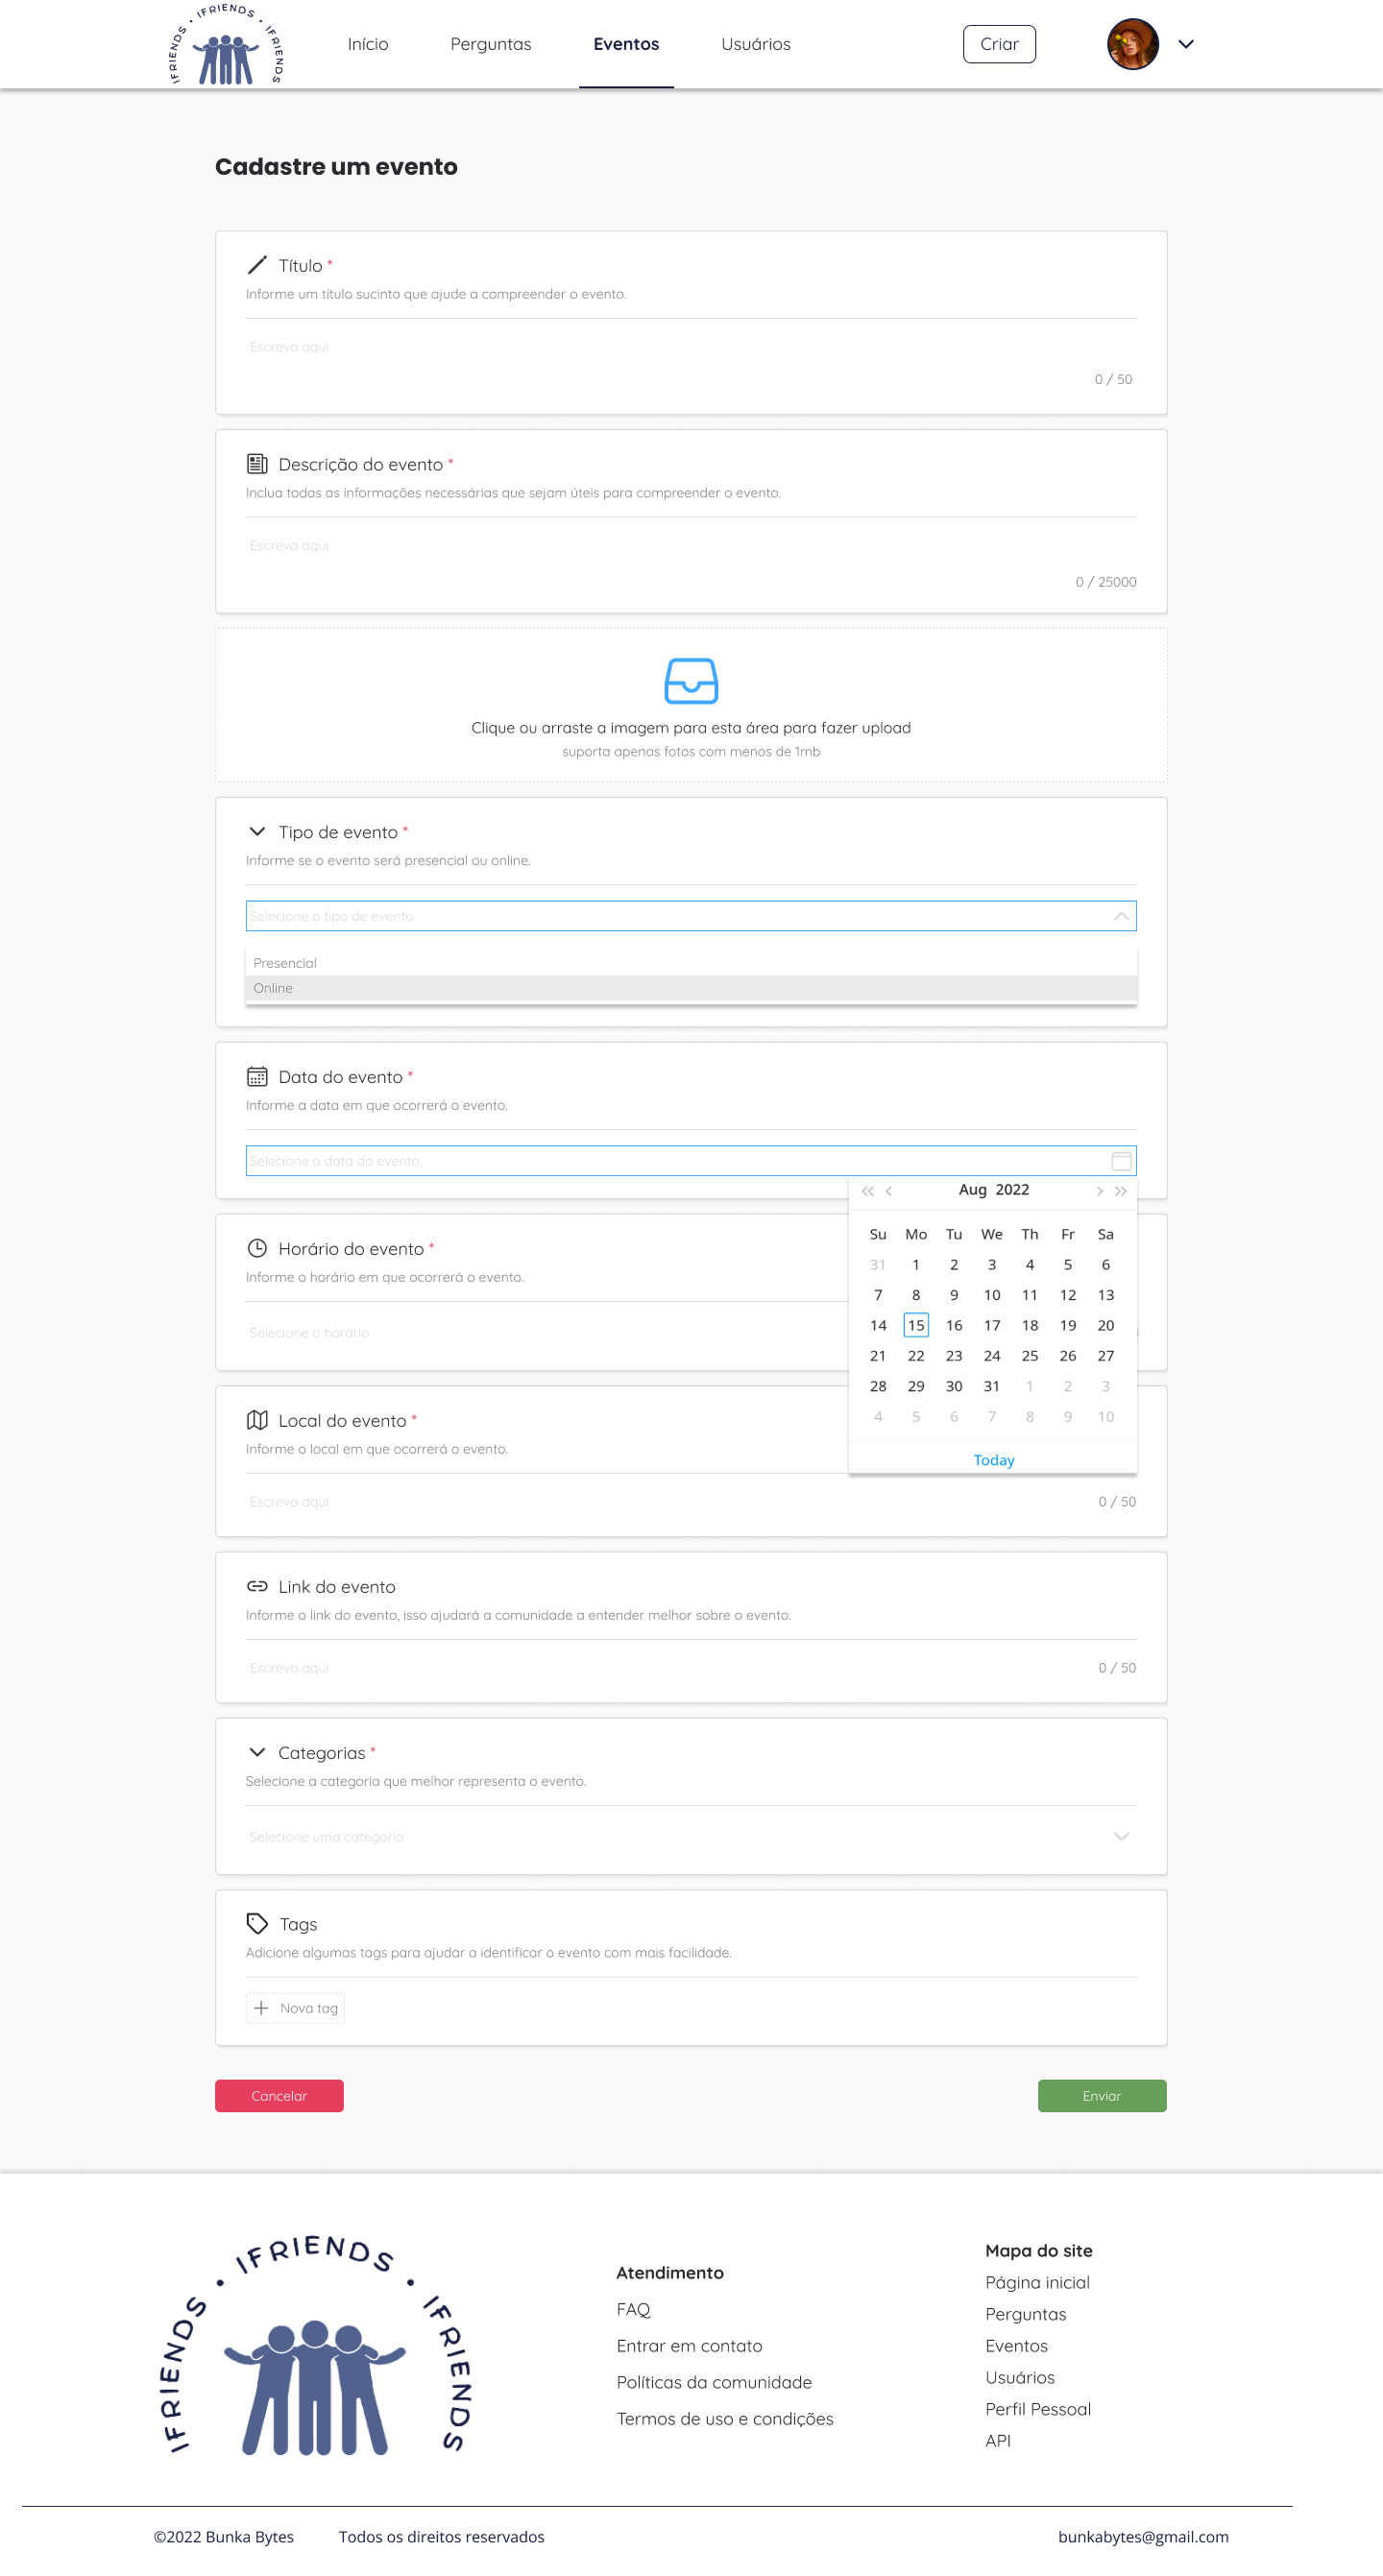
\includegraphics[width=0.8\textwidth]{anexos/Imagens_Prototipo/com_login/cadastro_eventos.png}
\fonte{Os autores.}
\end{figure}
\FloatBarrier

A \autoref{cl_usuarios} representa a página de usuários, nela o \gls{friend} pode visualizar ou pesquisar por usuários da comunidade. 

\begin{figure}[htb]
\centering
\caption{\label{cl_usuarios} Página de usuários}
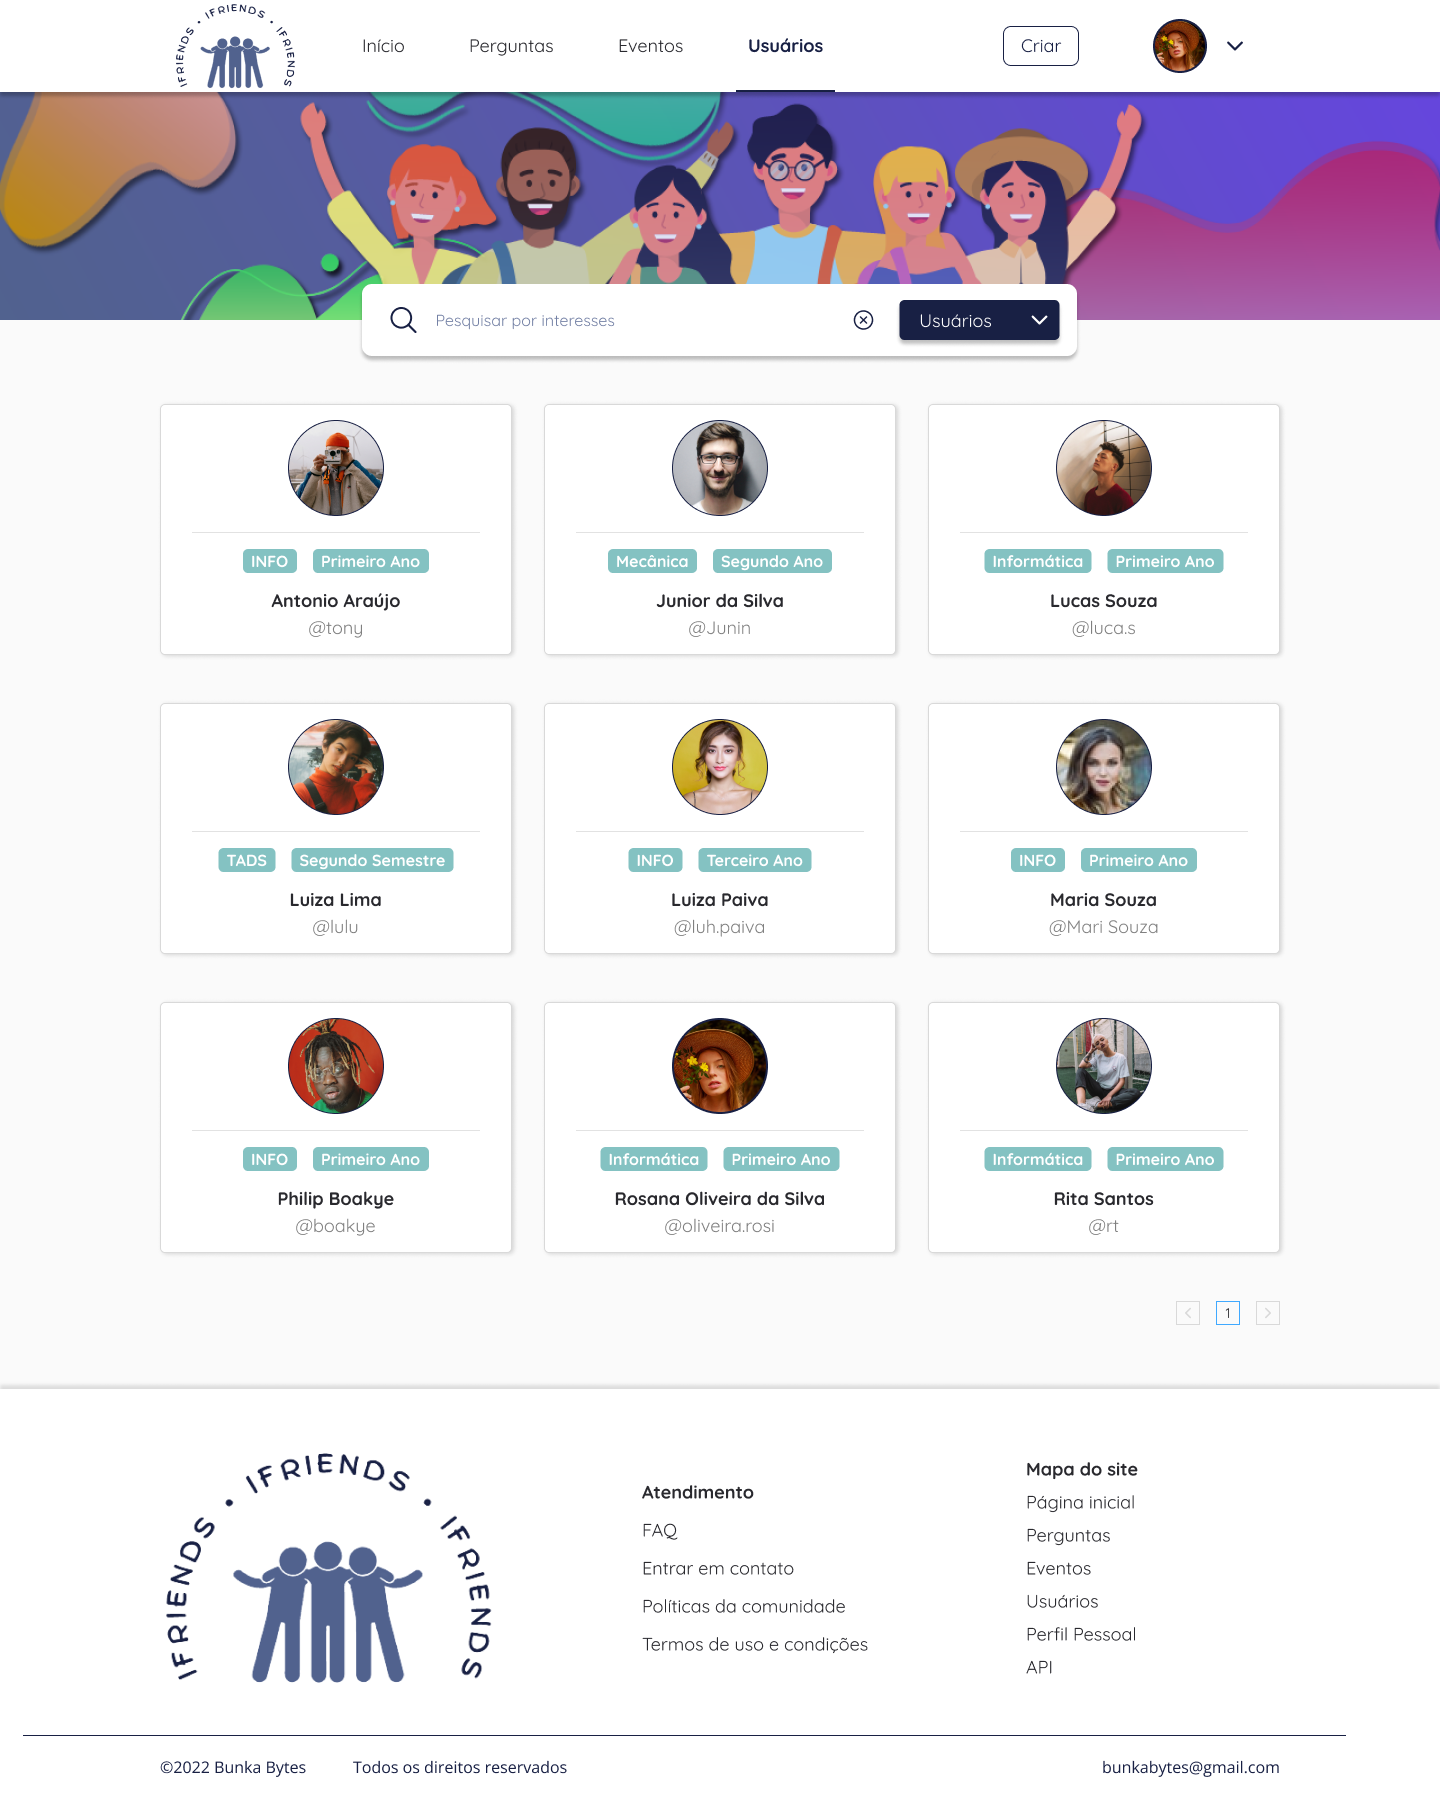
\includegraphics[width=0.8\textwidth]{anexos/Imagens_Prototipo/com_login/usuarios.png}
\fonte{Os autores.}
\end{figure}
\FloatBarrier

A \autoref{perfil_usuario} representa a página de perfil do usuário, nela são encontrados mais elementos sobre o \gls{friend}, como seus dados, a \gls{gamificação}, suas contribuições, ou seja, suas perguntas, suas respostas e os eventos que publicou. 

\begin{figure}[htb]
\centering
\caption{\label{perfil_usuario} Página de perfil do usuário}
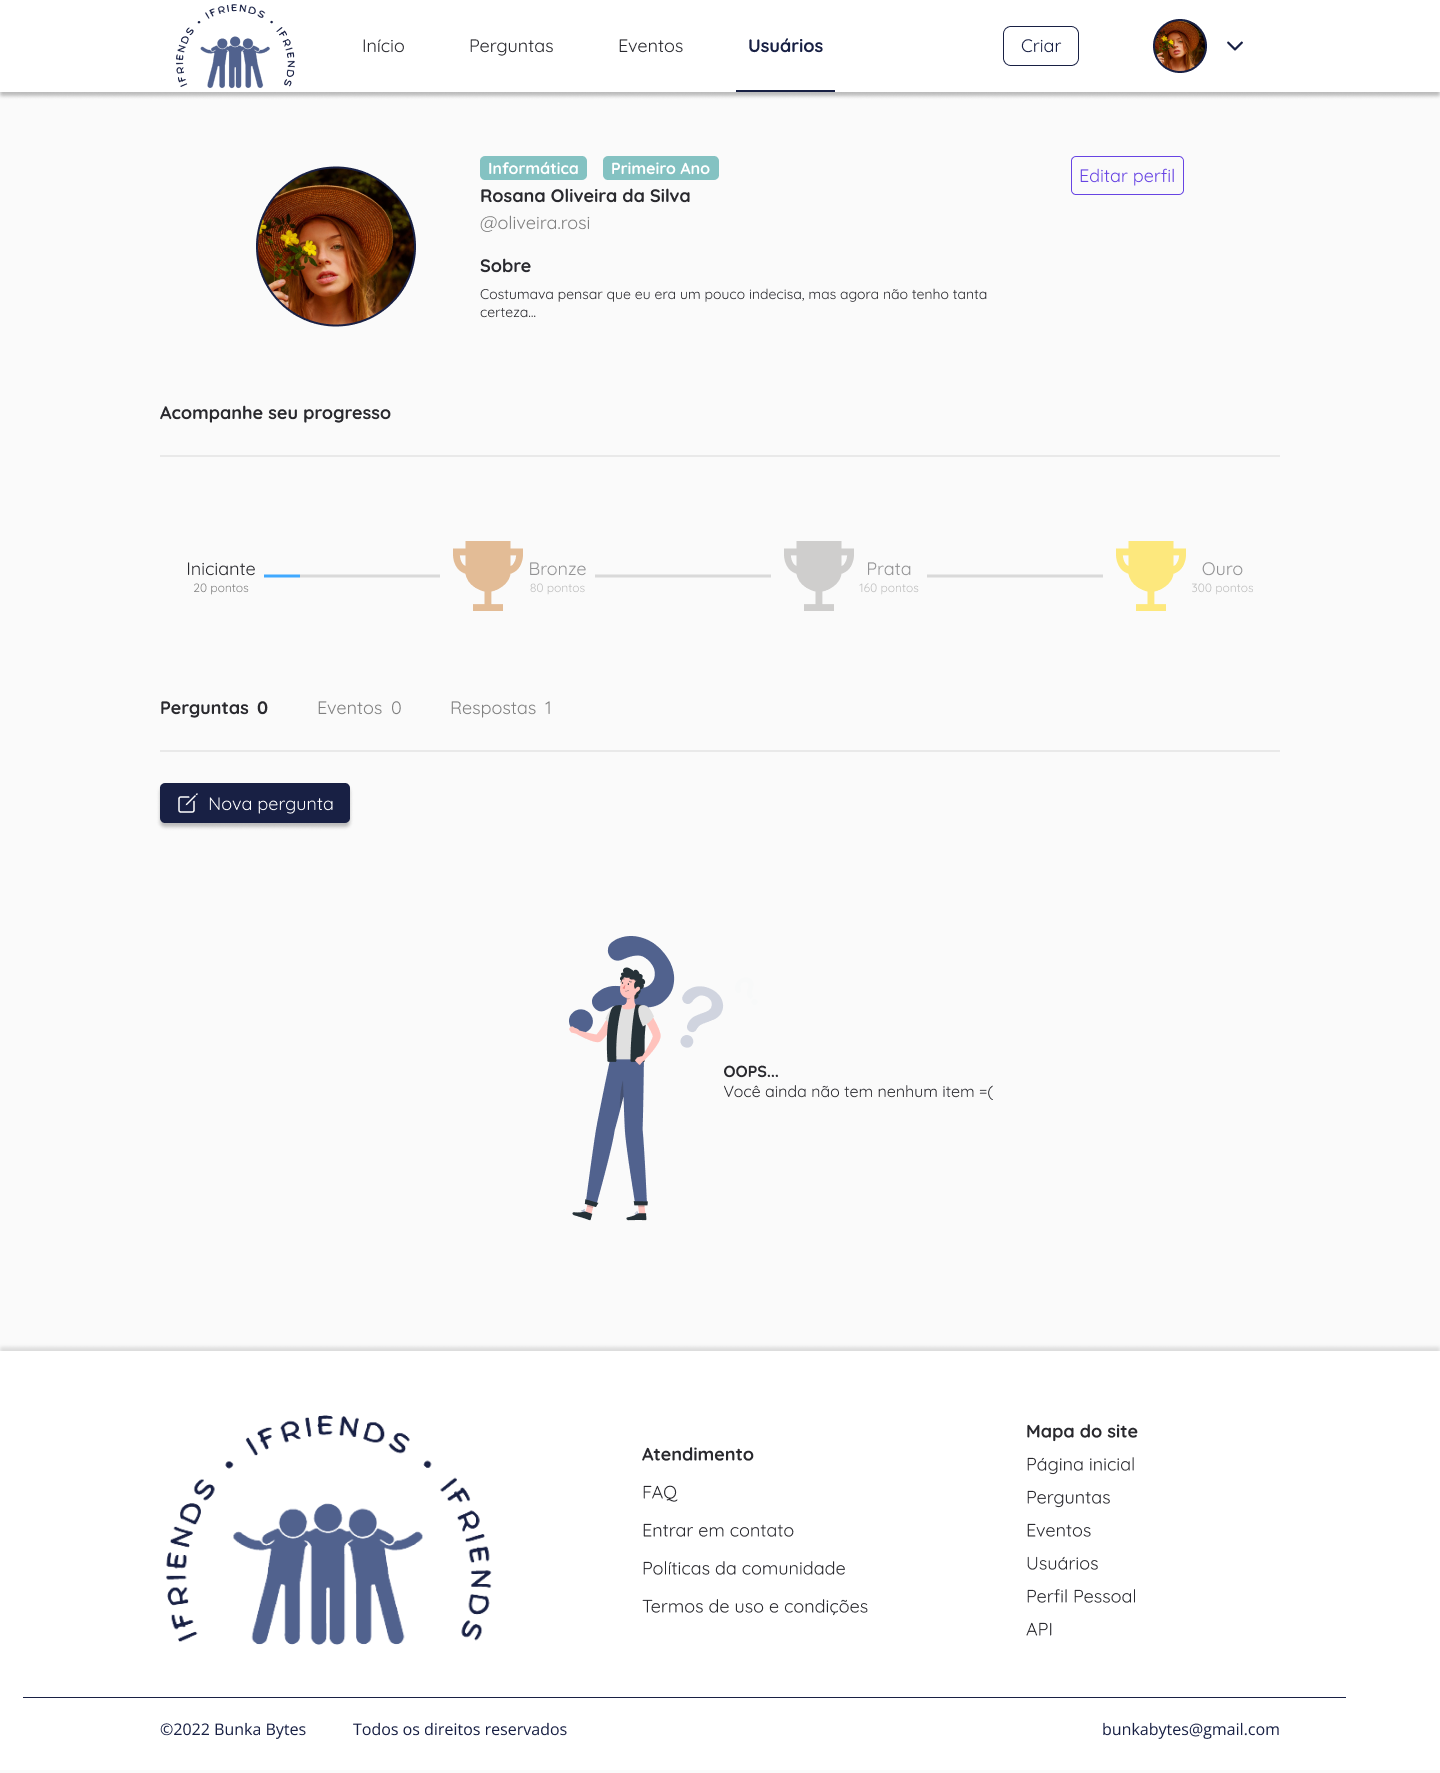
\includegraphics[width=0.8\textwidth]{anexos/Imagens_Prototipo/com_login/perfil_usuario.png}
\fonte{Os autores.}
\end{figure}
\FloatBarrier

Clicando no botão ``Editar perfil'' o \gls{friend} é direcionado a página para editar o perfil (\autoref{editar_perfil}).

\begin{figure}[htb]
\centering
\caption{\label{editar_perfil} Página de atualização de perfil}
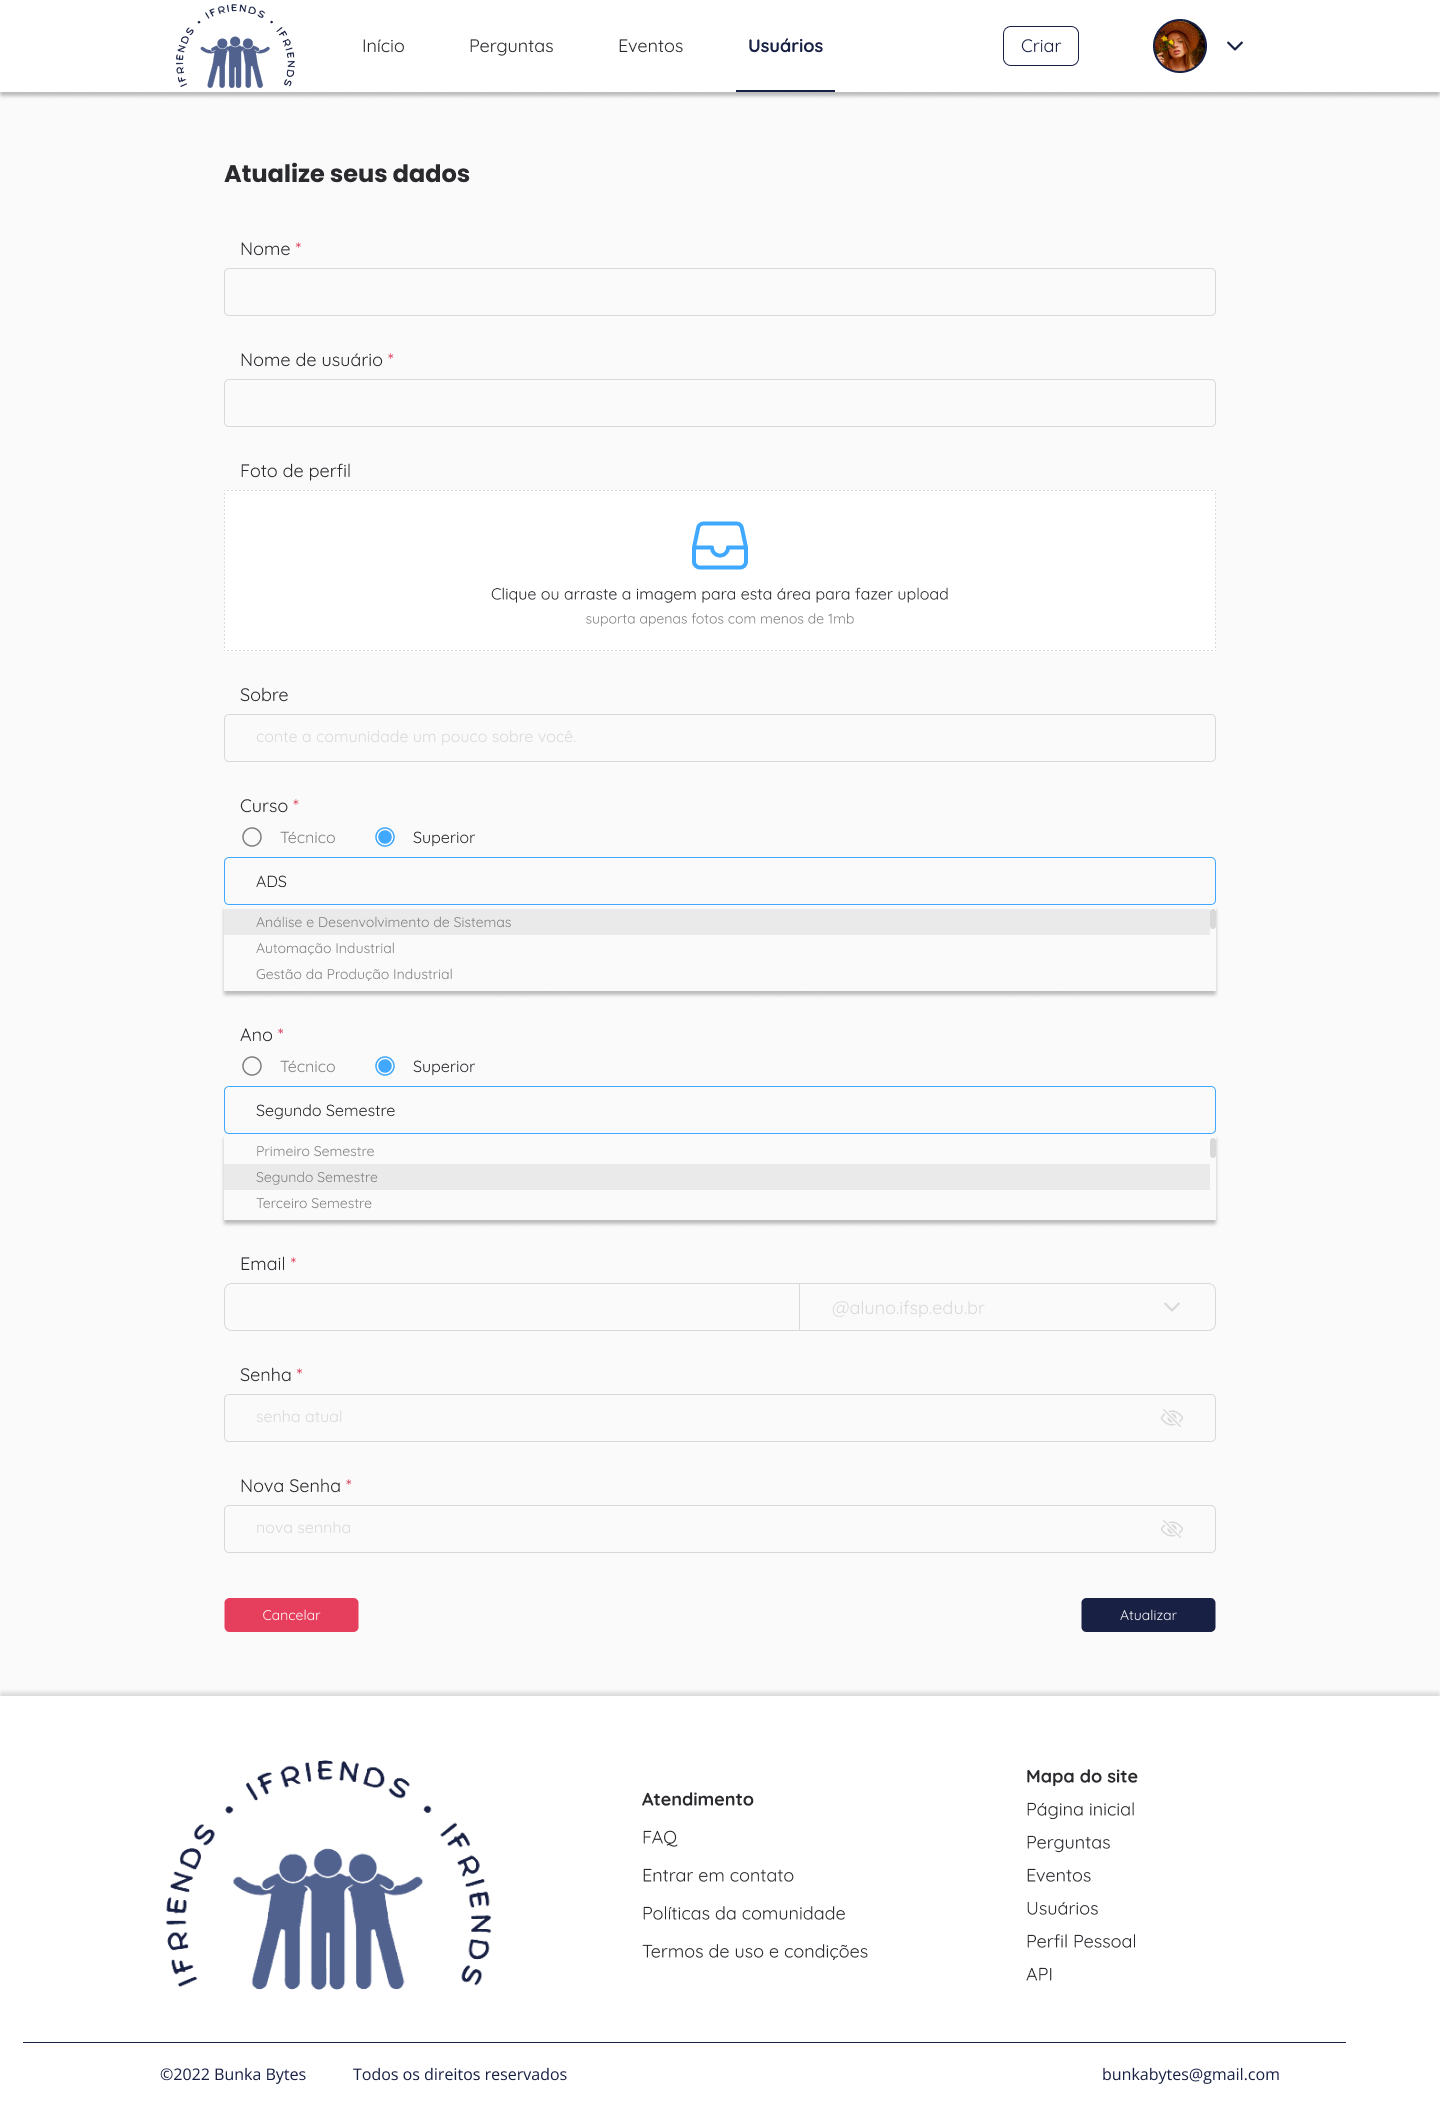
\includegraphics[width=0.8\textwidth]{anexos/Imagens_Prototipo/com_login/editar_perfil.png}
\fonte{Os autores.}
\end{figure}
\FloatBarrier

Vale ressaltar que as páginas prototipadas tem um fim norteador, logo pode ocorrer que alguns elementos não fiquem totalmente iguais. 